% Meaningful Substrates for Language Modeling (STLM)

\documentclass[11pt,a4paper]{article}
\usepackage[utf8]{inputenc}
\usepackage[T1]{fontenc}
\usepackage{hyperref}
\hypersetup{colorlinks=true, linkcolor=blue!70!black, citecolor=blue!70!black, urlcolor=blue!70!black,
  pdftitle={Toward Compulsory Scene-Mediated Language Modeling: Meaningful Substrates for Every Next Word},
  pdfauthor={Henrik Westerberg},
  pdfsubject={A research program for language generation through an obligatory, persistent configurational scene state},
  pdfkeywords={language modeling, scene-mediated generation, persistent world state, substrate-mediated reasoning, concept bottlenecks, grounded cognition, mental imagery}}
\usepackage{xcolor}
\usepackage{booktabs}
\usepackage{amsmath}
\usepackage{amssymb}
\usepackage{arxiv}
\renewcommand{\shorttitle}{Compulsory Scene-Mediated Language Modeling}
\usepackage{microtype}
\usepackage{tikz}
\usetikzlibrary{positioning}
\usepackage{graphicx}
\setlength{\emergencystretch}{2em}

\date{August 12, 2026}
\title{Toward Compulsory Scene-Mediated Language Modeling:\\Meaningful Substrates for Every Next Word}

\author{Henrik Westerberg\\Emergent Wisdom\\\texttt{henrik.westerberg@emergentwisdom.org}}

\begin{document}

\maketitle

\begin{abstract}
\noindent Can a language model build a world as it writes? The \emph{Substrate-Translated Language Model} (STLM) combines two commitments: a physical-and-schematic scene-state that evolves during free-running generation, and a compulsory per-token readout for which that state is the sole interface to lexical prediction. If meaningful targets share exploitable structure, they may promote reusable factors across words rather than independent token codes. We call the emergence of an accumulating, manipulable organization \emph{scene emergence}; it is the long-term hypothesis, not a result demonstrated here.

The stage-1 pilot tests this no-bypass prerequisite on a 1,024-token TinyStories vocabulary with one fixed pixel image or encoded description per token. Predictors emit substrate states from which stateless or causal-sequence readouts predict the next token. On the same 1,024 held-out contexts, causal description and pixel readouts reach 41.9\% and 37.8\% top-1 accuracy, below a direct-token model at 44.7\% but above stateless counterparts at 35.0\% and 27.8\% and a context-free frequency baseline at 8.1\%. The causal configurations differ in architecture, capacity, and supervision density, so their gains do not isolate history. Because each canonical can serve as an arbitrary codeword, the pilot establishes interface feasibility, not semantic use or scene construction. The immediate causal test is aligned versus permuted targets under matched conditions; compositional generalization and coherent responses to scene edits are later criteria.
\end{abstract}

\keywords{Language Modeling, Scene-Mediated Generation, Persistent World State, Substrate-Mediated Reasoning, Concept Bottlenecks, Grounded Cognition, Mental Imagery}

\section{Motivation}

The long-term proposal is not a language model that may consult an imagined picture when useful. It continuously constructs one internal state that accumulates what the unfolding text makes true, and every next-word decision must be read from that state. A couch contributes an object with spatial requirements; ``however'' contributes a contrast relation; a promise contributes agents, obligations, and possible violations. The state is intended to let these structures coexist and interact before they are translated back into words.

We use \emph{scene} in this inclusive sense: a joint configurational state containing physical entities and spatial relations, but also events, roles, mechanisms, constraints, and abstract schemas. Pixels or video provide a natural carrier for the physical part. Structured descriptions provide a second route: instead of depicting a word literally, they can keep its characteristic mechanism, relations, and consequences present at the interface. The destination is therefore broader than visual imagery, but narrower than an unconstrained hidden state: the representation must have externally specified structure that can be inspected, composed, and perturbed.

Scene construction and scene emergence are different claims. \emph{Construction} is this compulsory persistent-state architecture. \emph{Scene emergence} is the empirical hypothesis that, under it, locally meaningful structures will organize into a reusable joint model rather than remain a collection of private token codes. The stage-1 pilot does not yet maintain such a scene. It predicts independent, fixed canonicals at each position and tests the mandatory lexical seam needed before persistent construction can be attempted. Stage 3 (§5) is the first proposed implementation of the full scene-state.

Shared meaning could matter through reusable structure. Fifty thousand unrelated codewords present fifty thousand arbitrary associations. Meaningful targets can instead share factors: redness across objects, containment across scenes, paths across motions, opposition across arguments, and agent--action--consequence structure across mechanisms. If those regularities are present in the target family, a capacity-limited predictor may reuse them across many lexical decisions rather than memorize each target independently. On this account the substrate is not merely an information channel; it imposes a candidate inductive bias toward compositional, manipulable structure. For pixels, the strongest version requires context-specific generation or a medium-respecting spatial decoder. For descriptions, it requires targets whose relational and mechanism-level content matters beyond lexical identity. Fixed canonicals admit a codebook shortcut in both media.

Existing image-generation systems show that rendering objectives can learn reusable visual regularities such as boundaries, depth, containment, material, motion, and occlusion \cite{stablediffusion,flux2024,imagen2022}; description targets can extend the candidate structure to roles, rules, and consequences without depicting every abstraction literally. The toy does not test either proposed pressure: its single dense projection to one fixed target per word is invariant to coordinate permutation (§8.4), so it establishes a target-shaped interface rather than rendering or scene assembly.

The intelligence-relevant hypothesis is operational. We use \emph{substrate-mediated reasoning} to denote task-relevant computation that uses a substrate for three testable operations: \emph{composition}, by combining familiar factors in novel configurations; \emph{manipulation}, by changing a relation and propagating its consequences; and \emph{reuse}, by applying the same operations across unrelated content. A state that only converts one code into another does not qualify. Evidence additionally requires causal dependence: destroying intended structure impairs performance, while controlled semantic edits cause corresponding behavioral changes. This is a computational criterion and makes no claim about consciousness or human phenomenal imagery.

\paragraph{Coexistence as the proposed mechanism.} Every candidate update must remain compatible with the accumulated state. An object occupies space and preserves identity; a causal event constrains later consequences; a contrast relation requires two propositions in tension. Training against continued language would pressure inconsistent updates because they make later words harder to predict. This \emph{coexistence filter} is the proposed route from scene construction to coherence and first-principles reasoning: instead of recovering every implication anew from lexical associations, the model operates on structures already present together. Current models may already encode world structure implicitly; the experiment asks whether making a related state persistent, externally shaped, and obligatory changes behavior.

Architecturally, a large \emph{substrate predictor} (SP) reads running text and emits substrate states. A smaller \emph{token readout} (TR) maps only those states to tokens; it receives no token-side context channel. The substrate can be pictorial or descriptive, but in either case its target has internal axes and relations rather than being assigned as an unstructured token code. We use \emph{configurational} for this intended property. In the current stage, the single-state readout TR-S uses only the present state, while the causal readout TR-C uses the complete emitted 128-state window through the present position. Neither readout is the persistent scene of Stage 3: TR-C remembers an emitted trace, but it does not revise one accumulated world.

\paragraph{Evidence boundary.} The paper separates four claims. First, the \emph{operational claim}: TR-S and TR-C can recover context-dependent next-token information from SP outputs with no source-token context or token-side channel. The five-configuration pilot tests this claim. Second, the \emph{alignment claim}: the semantic organization of the target is load-bearing rather than interchangeable with an arbitrary code. This requires aligned-versus-shuffled and aligned-versus-random controls and is not tested here. Third, the \emph{fidelity claim}: emitted states remain on a human-interpretable configurational manifold rather than carrying token identity in subtle artifacts. The pixel strips diagnose this claim and show that gross visual content and machine decoding can diverge. Fourth, the \emph{scene-emergence claim}: a persistent state develops reusable physical-and-schematic organization that supports composition, manipulation, coherence, and transfer. That requires temporal state, matched baselines, structure-sensitive tasks, and causal interventions; it remains a research hypothesis.

\paragraph{Novelty boundary.} The ingredients are not individually new. Symbolic story systems have simulated worlds before verbalizing them; neural language models have maintained entity state; other systems generate scene graphs or images to guide text, retain persistent visual memories, or learn multimodal world latents \cite{talespin1977,dynamicentities2023,imagineverbalize2022,visualscaffolding2026,orca2026}. Concept Bottleneck Models and Large Concept Models already establish obligatory non-token interfaces at classification and sentence scales \cite{cbm2020,lcm2024}. The proposed novelty is the conjunction: free-running general language generation organized around one evolving physical-and-schematic scene-state that is the only interface available to every lexical decision, together with matched interventions that test whether the state's semantic organization matters. To our knowledge, prior work realizes subsets of this design but not that full combination. The novelty claim therefore concerns the proposed Stage 3 experiment; the present pilot demonstrates only its prerequisite interface.

\subsection{Reading with Mental Imagery}

The motivating analogy is human reading: narrative prose can prompt a reader to construct and revise a scene rather than retain only the surface wording. This analogy neither assumes that all reading is visual nor that STLM reproduces human imagery.

The cognitive-science literature provides context for this analogy. Barsalou's perceptual symbol systems \cite{barsalou}, Lakoff and Johnson's conceptual metaphor theory \cite{lakoff_johnson}, and the broader embodied-cognition tradition argue that abstract thought is built from imagistic and configurational primitives extended through metaphor to non-perceptual domains --- ``inflation'' through a flow metaphor, ``argument'' through a structure-of-physical-conflict metaphor, ``time'' through a metaphor of space. The architecture does not depend on this tradition being correct about humans. Its mechanistic proposals --- that rendering pressure encourages reusable decomposition, persistent coexistence pressure supports coherence, and explicit structure supports transfer --- are independent empirical hypotheses. The cognitive tradition is consistent with them, but cannot substitute for the controls and benchmark evidence described here.

\subsection{The Trajectory: Progressive Temporal Extent}

Many words encode \emph{characteristic time-shapes} that cannot be flattened into one moment without loss, while narrative coherence depends on longer trajectories --- an argument's arc, a relationship's trajectory, a discovery's progression --- that live across paragraphs. §4 develops the lexical case.

This observation shapes the research program: three stages that progressively extend the substrate's temporal extent, mirroring the visual-generation field's own path from still images to short clips to persistent scenes. \textbf{Stage 1} (§2--§3) emits one still representation per position: it handles object-shapes, flattens temporal content, and is the stage the toy of §8 implements. \textbf{Stage 2} (§4) replaces stills with short clips, so verbs and processes are represented natively and the representational pressure extends to event-shapes. \textbf{Stage 3} (§5) replaces per-position clips with a persistent multi-region scene-state --- the first stage whose substrate can hold discourse-level trajectory-shapes and filter each prediction against everything already accumulated. The commitment is to a substrate whose temporal extent matches what language actually encodes; each stage is a falsifiable experiment, not an assertion that the endpoint will work.

\subsection{The Empirical Question}

The empirical questions follow that progression. First: can a no-bypass substrate carry next-token information; do aligned targets beat shuffled and random ones; and do SP outputs preserve intended structure rather than only machine-readable identity? Next: do clips improve verb aspect, action coherence, and short-range temporal prediction beyond alignment-validated stills? Finally: does a persistent state improve long-context coherence, narrative-arc maintenance, character and object tracking, counterfactual manipulation, and abstract or relational language? The distinctive prediction is that gains, if any, will be \emph{coherence-specific and first-principles-specific} rather than uniform across benchmarks; §7 states the predicted profile and its falsifying signature.

Two natural media implement the intermediate substrate. The architectural commitment is to the intermediate layer between the two networks; its medium is a separate design choice. We test two implementations at toy scale (§8). The \emph{pixel substrate} uses a literal $64{\times}64$ RGB image, giving the target an explicit $(x,y)$ axis and making the SP's output directly displayable. The \emph{text-description substrate} encodes the same symbolic description through a frozen text encoder and keeps the per-token hidden-state sequence rather than pooling it. It is cheaper and preserves sequential position and contextual binding. Both implementations share the same authored descriptions. Only after within-medium alignment controls can their comparison test whether explicit spatial geometry contributes beyond ordered semantic structure.

The toy addresses only stage-1 interface feasibility. Both media carry decodable predictive signal, with descriptions outperforming pixels under fixed-canonical regression; §8.5 reports the complete-pipeline comparison and its limits.

\paragraph{Contributions.} The paper (i) states the meaningful-substrate hypothesis and its matched alignment test; (ii) defines STLM's compulsory, no-bypass lexical seam; (iii) develops the mechanism from still representations through event trajectories to persistent scene state; and (iv) implements a two-medium, five-configuration stage-1 pilot over a shared 1024-token TinyStories vocabulary, releasing its code, targets, per-example predictions, and reproducibility record.

\section{The Stage-1 Architecture}

The intended stage-1 architecture --- of which the toy in §8 is a restricted fixed-canonical regression specialization --- deploys two networks, both frozen at inference, separated by an explicit \emph{intermediate substrate}. The \emph{substrate predictor} (SP; large, the imagery engine in visual media) reads running text and emits a configurational representation at every position. The \emph{token readout} (TR; small, the pen) maps substrate states to tokens, either from the current state alone (TR-S) or from the causal emitted sequence through that state (TR-C). Neither scope receives source-token embeddings, an SP hidden state, or a parallel text pathway. A third artifact, the vocabulary $V$, is constructed once (§3) and shapes both networks; pixels, encoded descriptions, or other configurational representations can instantiate its medium.

\begin{figure}[ht]
\centering
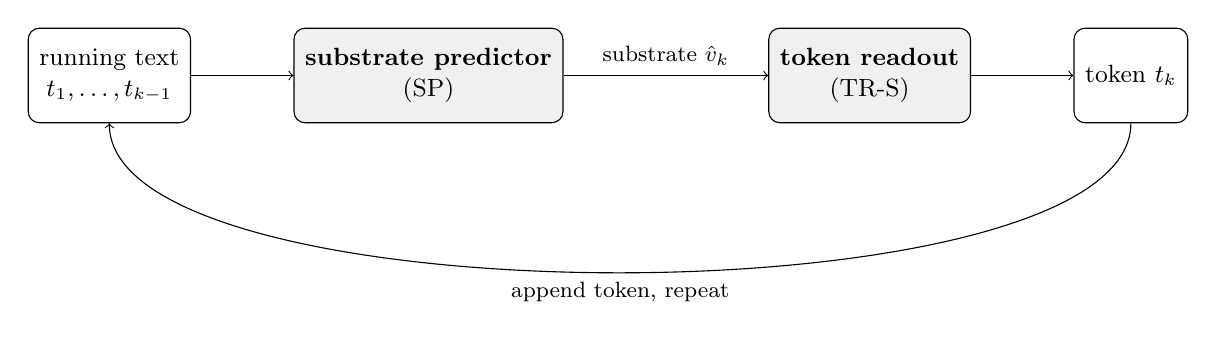
\begin{tikzpicture}[
  node distance=13mm,
  box/.style={draw, rounded corners, align=center, minimum height=12mm,
              inner sep=4pt, font=\small}
]
  \node[box] (ctx) {running text\\$t_1,\dots,t_{k-1}$};
  \node[box, fill=black!6, minimum width=25mm, right=of ctx] (sp)
        {\textbf{substrate predictor}\\(SP)};
  \node[box, fill=black!6, right=26mm of sp] (tr) {\textbf{token readout}\\(TR-S)};
  \node[box, right=of tr] (tok) {token $t_k$};
  \draw[->] (ctx) -- (sp);
  \draw[->] (sp) -- node[above, font=\footnotesize] {substrate $\hat v_k$} (tr);
  \draw[->] (tr) -- (tok);
  \draw[->] (tok) to[out=-90, in=-90, looseness=0.5]
        node[below, font=\footnotesize] {append token, repeat} (ctx);
\end{tikzpicture}
\caption{The stage-1 TR-S loop. At each position the substrate predictor (SP) reads the running text and emits a substrate state; TR-S names it as one token; the token is appended and the loop continues. The only channel between SP and TR-S is the current substrate state. The TR-C alternative freezes the same SP and trains a fresh causal readout over the complete 128-state window through the current position, still without source-token access.}
\label{fig:arch}
\end{figure}

\paragraph{The substrate vocabulary $V$.} A frozen mapping from token IDs to sets of vectors in $\mathbb{R}^d$. For each token $t$, $V(t) = \{p_1^t, \dots, p_n^t\}$ is a set of \emph{semantic prototypes}: images, video clips, encoded descriptions, or reconstruction latents that depict or encode plausible instances of $t$'s referent. For concrete tokens these may be many images or clips of the object or event; for abstract or function tokens they are LLM-authored image-schema or metaphorical instances. We write $\bar{V}(t)$ for the centroid, a summary statistic used only for analysis rather than as the training target (§3). The choice of encoder $E$ is the program's most consequential pre-training decision: the substrate inherits whatever geometry $E$ chooses to preserve. §9 returns to the choice between contrastive and reconstruction-objective encoder families.

A token's prototype set can be used in three increasingly strong ways. The simplest toy policy stores one canonical per word, making the SP a plain regressor to a fixed target. A frontier-scale \emph{random semantic-prototype} policy samples a fresh member of $V(t_k)$ whenever the next token is $t_k$, forcing the SP and TR to learn the whole semantic cloud rather than one point. A stronger \emph{context-selected semantic-prototype} policy chooses, for each training instance, the member of $V(t_k)$ that best matches the prefix context: the green apple in an orchard context, the bitten apple in a lunch context, the corporate-logo instance in a technology context. The selection step may use the prefix and the supervised target token during training, but it must not use future text or any side-channel unavailable to the SP at inference. Random selection tests whether the architecture can learn a word's prototype distribution; context-selection tests whether the substrate can carry the situated meaning of this particular occurrence. These are different experiments and should not be conflated.

\paragraph{Substrate predictor (SP).} A large text-conditioned generative model. Its input is the text prefix with full long context; its output at every position is a single substrate state $\hat{v}_k \in \mathbb{R}^d$ \emph{sampled} from its learned distribution over plausible next-word representations. Architecturally it is a causal transformer with a generative head --- diffusion noise prediction in $\mathbb{R}^d$, or autoregressive prediction over a discretization of $\mathbb{R}^d$ --- not a regressor at frontier scale. §3 explains why this matters: a regressor trained against a multi-prototype set collapses to its conditional mean, washing out the per-instance structure the substrate is meant to carry; a generator trained on sampled or selected prototypes learns the distribution and emits crisp instances. After training the SP is frozen.

\paragraph{Token readout (TR; the pen).} A learned function that maps the SP's emitted substrate representation into a distribution over tokens. TR-S is a stateless map $f_{\mathrm{S}}: \mathbb{R}^d \to \Delta^{|\text{vocab}|}$ invoked once per generated token; it receives only the current per-position substrate $\hat v_k$. In the reported toy comparison, TR-C is a causal sequence map: a medium-specific state adapter, shared over time, independently maps each $\hat v_j$ to 256 dimensions; a two-layer, eight-head causal Transformer maps $(\hat v_1,\ldots,\hat v_k)$ to vocabulary distributions at every aligned position. Its position-$k$ decision can depend on substrate states $\hat v_{\leq k}$, including the current state, but it receives neither the original token prefix nor an SP hidden state. TR-C is freshly initialized and trained as a complete readout rather than as an adapter to TR-S. For one grid state TR-S can be a CNN; for a description state it can be a small transformer over the substrate's internal positions.

Conceptually, the division of labour mirrors §1: the SP has \emph{already produced} the substrate representation, and the TR performs the modality conversion into the lexical form the output stream requires. A TR is functionally specialized to its own SP's substrate idiom rather than being a generic decoder of arbitrary states; §3 separates its training regimes. The architectural constraint is that no TR receives a text-context side channel. For TR-S, predictive sufficiency must rest on the current SP output; for TR-C, it may rest on the causal substrate sequence through the current state.

\paragraph{The readout seam.} One substrate state and one readout invocation occur per generated token, and no substrate state is revised after emission. This constrains the interface, not the SP's internals --- a diffusion or autoregressive head may run many internal iterations to produce one state. Crucially, each $\hat v_k$ is understood throughout as a \emph{positionally or configurationally structured} representation --- a pixel grid, a video clip, an encoded-description sequence, or another object with internal positional and relational content --- not a single global compression. An explicit spatial axis is additionally required for the architecture's spatial-reasoning claims; §9 elaborates.

\section{Stage-1 Training}

Stage 1 separates construction of the intended substrate organization from learning the two sides of the lexical seam. Phase zero builds and freezes the substrate vocabulary; phase one teaches the token readout to recognize states from that vocabulary; and phase two teaches the substrate predictor to generate an appropriate next-token state from linguistic context. Keeping these roles distinct makes it possible to study readout fidelity, adaptation to predictor outputs, and optional end-to-end coupling as separate design choices.

\subsection{Phase Zero: The Visual Vocabulary}

The visual vocabulary is computed once before model training. For each token, generate hundreds of varied visual descriptions (for concrete tokens, scene contexts like ``a red apple on a wooden table''; for abstract tokens, metaphorical descriptions via an LLM-as-dictionary step; for function tokens, glyph descriptions or substitute-word descriptions). Phase zero uses three distinct maps. A description substrate applies a frozen \emph{text} encoder, $d_t \mapsto E_{\text{text}}(d_t)$. A pixel substrate applies a text-conditioned \emph{generator}, $d_t \mapsto G(d_t) = I_t$. A latent substrate additionally applies an \emph{image} encoder to the rendered result, $I_t \mapsto E_{\text{image}}(I_t)$. A text encoder produces a conditioning representation rather than an image or spatial image latent. Cache the resulting prototype set and its centroid per token.

Costing this stage at frontier scale requires an explicit throughput analysis. A 50k-token vocabulary at 500 prototypes per token means 25 million prototypes: cheap if the final step is a batched text-encoder pass, but dominated by description authoring and, for pixel or latent substrates, by rendering --- the 1,021 rendered lexical images for the vocabulary of §8 alone took roughly 14 hours on one laptop (the other three canonicals are fixed special-token sentinels). A frontier estimate must state generator and encoder throughput, representation precision and dimensionality, resulting storage, and deduplication and validation cost. The resulting vocabulary file is read throughout training and retained only as a reference afterward; neither the phase-zero auxiliary LLM nor the encoder is retained after construction.

\subsection{Phase One: Training the Token Readout}

Standard multi-class classification on the vocabulary alone, with no text corpus. Sample (prototype, token) pairs from the vocabulary and train the TR with cross-entropy to output the correct token. The TR learns to recognize the entire prototype cloud per word, not just the centroid. After phase one it has prototype-recognition competence over $V$. In phase two (§3.3) it is then either frozen, continued in lockstep on freshly sampled prototypes, or trained directly on the SP's actual outputs --- three design points along the readout-training axis, trading off convergence stability against the human recognizability of the SP's emitted substrates. The TR-S/TR-C distinction is orthogonal to this axis: either scope can be trained on actual SP emissions, but TR-S learns from individual states whereas TR-C learns from causally masked sequences with an aligned loss at every position.

The choice also decides what the TR can exploit, and three mechanisms must be kept apart. When a TR is trained after a frozen SP on that predictor's actual emissions --- the option the toy of §8 takes --- it can adapt to stable deviations and artifacts in the SP's output distribution. Because the SP is frozen and no gradient crosses the seam, this is \emph{one-way decoder adaptation}, not mutual co-adaptation: the readout moves toward the predictor, never the reverse. \emph{Joint private coding}, in which the pair settles on a shared convention that need not respect the targets' meaning, becomes possible only under an end-to-end objective in which readout gradients reach the SP --- the optional coupling term §3.3 reserves. A third regime trains the TR only on authored canonicals, making it a \emph{fidelity diagnostic}; it constrains the SP only if its loss is included in the SP's objective. Under the no-gradient scheme specified here it is a measuring instrument rather than a training pressure. This independence creates distribution shift because a canonical-only reader never sees SP drift. Meaningful within-concept variation (§9), rather than exact canonical points, is therefore required for a semantic reader.

The TR is intended to be small (1--10M parameters) and is never exposed to source tokens directly; at toy scale TR-S trains in minutes, though a 50{,}000-way classifier over 25 million prototypes would not. The restriction still permits both readouts to learn token priors and exploit label-correlated artifacts because they see token labels and their empirical frequencies during training. TR-C can additionally model regularities across a causal substrate sequence, including language regularities encoded there indirectly. The architectural guarantee is the absence of a token-side context pathway, not the absence of all lexical statistics or contextual information.

\paragraph{Why a learned token readout, not a lookup table.} A TR could in principle be replaced by a brittle nearest-prototype lookup: given a substrate state $\hat v$, return the token of the canonical prototype it most closely matches. This degenerate alternative fails because the SP's emitted substrates are not database entries. The SP produces approximate, drifting, occasionally out-of-distribution states --- a description like ``a small red round thing with a leaf'' instead of the canonical ``a red apple on a wooden table,'' or a pixel image with blurred edges and shifted positions. A nearest-prototype rule always returns the closest stored class, but it partitions the representation space into exactly the Voronoi cells induced by the stored prototypes under the chosen metric. It cannot learn invariances or boundaries that depart from that geometry, whereas a learned TR can model non-Voronoi boundaries and the systematic transformations present in the SP's actual output distribution. (An $\langle$unk$\rangle$ or abstention outcome is not a property of nearest-neighbour classification at all: it would require a separately specified rejection threshold.) The TR exists precisely to be a \emph{tolerant reader} of the noisy substrate the SP actually produces: a learned function that maps a \emph{manifold} of SP emissions around each canonical to the same token. This is why the program prefers, both at frontier scale (the full prototype set $V(t)$) and in the toy (§8: TR trained on the SP's actual outputs), training schemes that expose the readout to substrate variation rather than to canonical points alone. The TR must learn the fuzzy inverse of the canonical mapping, not the brittle one.

\subsection{Phase Two: Next-Image Prediction}

Conditional generative training over the substrate vocabulary. For each position $k$, the policy defined in §2 supplies a target $p_k \in V(t_k)$. The substrate predictor reads the prefix $t_1, \dots, t_{k-1}$ and is trained against $p_k$ with diffusion noise prediction or autoregressive cross-entropy over a discretization. Random selection teaches the full conditional distribution $p(\hat v \mid t_{1:k-1})$ over a word's prototype cloud; context selection teaches the contextually appropriate instance.

This objective choice is consequential. MSE regression onto a fixed target (the centroid), or even onto resampled prototypes, collapses to the conditional mean --- a probability-weighted blur of all plausible next-word images. A generative objective with resampled targets matches the distribution rather than its average, so the predictor's emitted substrate is a crisp specific instance rather than a smeared superposition. This matters most for relational and abstract terms, whose per-instance visual variation is largest and whose means are therefore the most washed-out.

\paragraph{What fixed-target regression computes.} The collapse has an exact characterization, and stating it also bounds what a feasibility result can mean. Let $c_y \in \mathbb{R}^d$ be the canonical target for token $y$, and let $C$ be the matrix whose rows are those canonicals. A predictor minimizing squared error against $c_Y$ has Bayes-optimal deterministic output
\[
  g^*(x) \;=\; \mathbb{E}\!\left[c_Y \mid X = x\right] \;=\; \sum_y p(y \mid x)\, c_y \;=\; C^{\top} p(\cdot \mid x),
\]
the posterior-weighted average of every plausible next word's canonical. Four consequences follow. First, blurring is not an implementation defect but the objective's optimum: under next-token uncertainty the best fixed-target output \emph{is} a superposition. Second, if $C$ has full row rank the posterior is in principle recoverable from $g^*(x)$ by a linear map, so a readout can succeed even when the canonicals carry no meaning at all. Third, seam feasibility is therefore weak evidence by itself: the pixel substrate offers 12,288 coordinates and the flattened description substrate 21,504 for only 1024 classes, so either target set has ample room to act as an error-correcting output code \cite{ecoc2019}. Fourth, semantic alignment cannot change what is expressible through such a channel; it can only change the inductive bias --- which functions are cheap to learn, how they generalize, and how they transfer compositionally. This is precisely why the central claim is posed as a question about sample efficiency and transfer under a permutation control, rather than about whether the seam can carry information.

This exact linear characterization applies to the pixel condition, whose loss is squared error on unconstrained outputs. The description condition instead applies a per-position cosine loss to unit-normalized outputs, so its optimum at slot $j$ is the \emph{normalized direction} of the corresponding conditional mean, $g_j^*(x) \propto \sum_y p(y \mid x)\,\bar c_{y,j}$ with $\lVert g_j^*(x)\rVert = 1$. Because each slot discards magnitude separately, full row rank of the raw flattened description matrix no longer guarantees that the token posterior is linearly recoverable, even though the mapping can still carry substantial class information.

This characterization also makes the target matrices worth measuring directly, which costs no training. We summarize each by the participation-ratio effective rank of its singular spectrum, $\left(\sum_i \sigma_i\right)^2 / \sum_i \sigma_i^2$, which counts how many singular directions carry the variance. Flattened, the pixel canonicals form a $1024 \times 12{,}288$ matrix (values scaled to $[0,1]$) and the description canonicals a $1024 \times 21{,}504$ matrix; the stored description states are already per-position unit-norm, as the seam requires, so that normalization leaves their spectrum unchanged.

\begin{center}\small
\begin{tabular}{lrr}
\toprule
Target set & Uncentered & Mean-centered \\
\midrule
Pixel canonicals       &  57.9 & 193.0 \\
Description canonicals & 564.3 & 769.0 \\
\bottomrule
\end{tabular}
\end{center}

\noindent Preprocessing matters: uncentered, the description set spreads its variance over roughly ten times as many directions as the pixel set, but after removing the mean the ratio falls to about four. All 1024 pixel canonicals are distinct, so the concentration is not duplication; it is consistent with strong shared image statistics --- a common mean image, global brightness and colour cast, broad layout --- across independently rendered scenes, though we have not inspected the leading singular vectors to confirm that reading. Effective rank does not measure numerical conditioning: the description target set is higher-effective-dimensional, but not necessarily better conditioned. Even so, a less concentrated output code is a candidate explanation for the medium gap reported in §8.5 that is independent of meaning, and it should be controlled before any medium comparison is read semantically.

Returning to the training procedure, in lockstep --- same step, same target $p_k$ --- the TR is trained on $(p_k, t_k)$ with cross-entropy, with one optimizer per network and no gradient crossing the seam. The shared per-step prototype is a data anchor, not an optimization coupling: the SP sees $p_k$ as generative target, while the TR sees $p_k$ as classification input. The lockstep is preserved deliberately: it reserves the seam for an optional end-to-end coupling term $\text{CE}(f(\hat v_k), t_k)$ to be introduced later without restructuring the training pipeline. We call the objective \emph{next-substrate prediction}; stage 1 specializes it to images, stage 2 to video, and the text-description toy to encoded description sequences. At deployment, the frozen SP and TR run in series; no training-only component participates in inference.

\section{Proposed Stage 2: Next-Video Prediction}

Stage 2 enriches the substrate from still images to short videos. The architecture's structural shape is unchanged --- the SP reads text, emits a substrate state, and the TR names it as a token --- but the substrate at each position is now a short video clip rather than a single image.

Many words are not static. ``Threw'' is a trajectory --- a grasp, a wind-up, a release, a flight, an arrival; ``melted'' is a solid-to-liquid transition; ``collapsed'' is a process with a before and an after. Even ``door'' carries the dynamic of opening and closing, while ``bridge'' carries the affordance of crossing. A still image can capture only one moment of this time-structure; flattening a verb, process, or transition into a single configuration is intrinsically lossy in a way depicting a roughly time-invariant table is not. A video substrate instead represents trajectories and transitions across frames --- the throw's motion, the melting, the door's swing --- so its expressive capacity better matches what these words encode.

The vocabulary stores short video clips per token or, more practically, sequences of vectors in a video encoder's geometry. Vocabulary construction uses a text-conditioned video \emph{generator} to render each clip and that generator's autoencoder to represent it --- the components of systems such as Stable Video Diffusion \cite{svd2023} or Sora \cite{sora2024} --- rather than an image pipeline.

The empirical question is whether extending the substrate's temporal capacity from one moment to a clip-sized window measurably reduces the failure modes that still images cannot handle. Stated precisely, stage 2 tests whether \emph{temporally structured targets improve temporally structured prediction}. Stages 1 and 2 supervise each position against an independently chosen next-word canonical, so neither implements substrate-level coexistence; that property first appears in the persistent state of stage 3 (§5). The SP's transformer state necessarily conditions on the prefix, but this is ordinary contextual prediction rather than an explicit substrate-level compatibility operation. The empirical prediction is that stage 2 outperforms stage 1 on tasks where verb-aspect, action-sequencing, and short-range temporal-trajectory matter, while remaining comparable on tasks dominated by static configurations.

\section{Proposed Stage 3: Persistent Scene Construction}

Stage 3 is the intended endpoint: free-running generation maintains one continuously updated configurational scene-state across the discourse, and the token readout receives only a state selected from it. The scene is not a sequence of independent pictures or an optional memory retrieved when useful. Each generated word updates the same working state; later lexical decisions must therefore be compatible with what has accumulated. This is the proposed \emph{coexistence filter}. Stage 3 has not been implemented, and the stage-1 pilot contains neither scene accumulation nor scene-level compatibility pressure.

The intended scene carries both \emph{physical/visual content} (the running boy, the kitchen layout, the light) and \emph{schematic/configurational content} (relations, abstractions, image schemas \cite{lakoff_johnson} --- containment, support, path, balance, force, contrast) in one working state. The distinction is functional rather than a literal architectural partition. Both kinds of content are subject to the same compatibility pressure: a candidate ``however'' must fit the contrast structure already present, while a candidate ``couch'' must fit the spatial structure.

\paragraph{Scene contents and organization.} The scene maintains a video-like internal representation of what the text describes spatially --- objects, layout, motion, light. New text causes the scene to extend: the boy walks across the room, the light shifts, the door opens. The structure is preserved in the predictor's working state, not rendered to pixels at inference (that would be prohibitively expensive), but maintained internally in the kind of representation produced by frontier video world models. Spatial coherence is enforced by coexistence: an object placed in the scene takes up space, occludes things behind it, has consistent material properties; subsequent text whose configurations would break this spatial coherence is pressured against by the substrate.

The same scene-state also carries content that has no straightforward visual instantiation --- relations, abstractions, image schemas. ``However'' has no visual referent, but it has a \emph{schematic} referent: contrast, reversal, two propositions in tension. ``The argument collapsed'' is comprehensible because the schema of collapse is present, not because anything visual is happening. ``Inflation'' lives as a flow-or-expansion schema; ``time'' as a path schema; ``equality'' as a balance schema. These configurations live in the same scene-state as the physical content. They are not pictorial but they are \emph{configural} --- they have geometry in the encoder's space, they compose with each other and with the physical content, and they are subject to the same coexistence-filtering. The schematic content is what lets the substrate carry trajectory-shapes (a developing argument, a betrayal's stages, a discovery's progression) across the generation: these shapes are extended over time, not single moments, and the persistent scene is what holds them.

Word prediction at each position draws from whichever aspect of the scene the upcoming word's referent depends on. A position whose next word names a concrete object reads off the physical content; a position whose next word is ``however,'' ``although,'' or ``would have been'' reads off the schematic content. The TR sees a representation pulled from the appropriate part of the scene and names it. The architecture does not pre-designate which content category a given word lives in: the SP learns the joint structure during training, and the readout is shaped by the same training signal that shapes the rest of the system. Paivio's dual-coding theory \cite{paivio} and Lakoff's image schemas \cite{lakoff_johnson} provide broad motivational precedents for distinguishing imagistic, verbal, and schematic forms of representation, though neither describes two such content kinds coexisting in one learned latent. These theories motivate the distinction but are not assumptions of the architecture.

The architecture leaves physical and schematic content distributed within one latent rather than assigning them separate regions. We \emph{hypothesize} that a joint objective requiring both kinds of content --- video reconstruction for physical structure, language readout including abstract and relational terms for schematic structure --- would yield functionally distinguishable representations of the two, because the two prediction tasks reward different geometric properties. They could be distributed, superposed, nonlinearly separable, or related by an arbitrary rotation rather than occupying literal or axis-aligned sub-regions. Both separability and causal specialization would have to be measured, and probe separability alone would not show that the model uses the distinction; the abstract--physical composition test under H5 (§7) therefore requires causal intervention rather than geometric distinguishability.

\paragraph{What stage 3 tests.} Stage 3 is hypothesized to improve several capabilities that remain unreliable in current token-based language models. Empirical predictions: stage 3 should handle narrative coherence across long text spans (the boy who entered the room in chapter one is still there in chapter three) because the scene maintains him; counterfactual reasoning by scene-manipulation (what if the boy hadn't picked up the key) because the scene can be perturbed and the consequences read off; theory of mind through imagined embodiment (placing oneself in another's scene position) because the scene supports perspective-taking as a substrate operation; common sense by exploiting joint physical-and-schematic content (ice melts because the melting trajectory is a substrate object; betrayal hurts because the trust-and-rupture schema is a substrate object); and abstract/relational language without per-token metaphor workarounds, because the schematic content lives in the scene alongside the physical content. The architectural prediction is that these gains emerge as side-effects of the coherence-filtering mechanism operating over a persistent scene.

\paragraph{Open design problems.} Implementing Stage 3 requires explicit machinery for maintaining and updating the scene across positions, analogous to persistent video world models. Candidate carriers include a video-codec-like internal representation or a sufficiently large hidden state with temporal attention over scene history. Beyond that, a concrete architecture must specify how the per-position readout selects the relevant part of the scene without reintroducing an unrestricted hidden-state pathway; which loss anchors the persistent state to externally specified meaning rather than letting it drift into an arbitrary recurrent code; why physical and schematic content should occupy separable regions rather than an entangled rotation of the latent; how token probabilities are defined when the predictor samples stochastically, and how iterative (for example, diffusion) sampling coexists with the one-state-per-token loop; and what the inference cost per generated token is. Together, these questions define the central technical agenda for stages 2--3.

\section{Related Work}

The relevant prior work is best separated along three axes: whether a non-token representation is an \emph{obligatory route} to lexical output, whether generation maintains an \emph{evolving scene or world state}, and whether the state's \emph{semantic organization} is tested causally. Prior systems realize important subsets of this program. Stage 1 isolates the compulsory per-token seam; the proposed Stage 3 combines that seam with one persistent physical-and-schematic scene and matched semantic interventions. To our knowledge, no prior free-running natural-language system combines all three.

\subsection{Concept Bottlenecks and Representation-Space Language Models}

Concept Bottleneck Models first predict human-specified concepts and then make the final task prediction only from those concepts \cite{cbm2020}. This is the clearest architectural precedent for an obligatory, inspectable seam. CB-LLM applies the pattern to large text-classification benchmarks using automatically generated textual concepts \cite{cbllm2024}; CB-pLM places an interpretable concept layer before token prediction in a generative masked protein language model \cite{cbplm2024}. These systems establish both the two-stage commitment and its application to language-model outputs, although they do not study left-to-right natural-language generation through per-token visual or description canonicals. Subsequent work showed that CBM intermediates leak task information beyond the intended concepts \cite{cbmleakage2022}; the channel-versus-meaning distinction that motivates our controls is the generative analogue of that finding.

Large Concept Models (LCMs) are the closest broad precedent \cite{lcm2024}. An LCM autoregressively predicts the next sentence in a fixed SONAR embedding space and uses a frozen SONAR decoder to reconstruct text. It therefore already demonstrates language generation through an obligatory meaningful representation and a decoder that does not receive the original token context. Continuous Autoregressive Language Models similarly predict reconstructable continuous vectors for multi-token chunks \cite{calm2025}. At token granularity, Projected Autoregression makes continuous next-token vectors the primary autoregressive interface, studies how embedding geometry affects stability, and commits outputs by nearest-neighbor projection \cite{projectedar2026}. Earlier continuous-output sequence models already predicted word embeddings in place of a softmax \cite{vmf2019} or used error-correcting output codes for sequence prediction \cite{ecoc2019}; these are important alternative explanations for why structured continuous targets can help, independent of any configurational reading. Next-concept prediction learns discrete multi-token semantic units and predicts them alongside ordinary tokens \cite{nextconcept2026}, sharing the goal of routing prediction through semantic units while retaining the token pathway.

Continuous and concept-space language generation are established precedents: LCM supplies obligatory sentence-space generation, while Projected Autoregression studies learned or pretrained token-embedding geometry and commitment dynamics. STLM's narrower proposal uses externally authored modality-derived organization, extends it toward a persistent scene-state, and holds the target set fixed while permuting word-to-substrate alignment to test meaning causally.

\subsection{Visual Supervision and Machine Imagination for Language}

Vokenization contextually associates each language token with a related retrieved image and uses the resulting ``vokens'' as visual supervision \cite{vokenization2020}. VaLM retrieves images for each textual context and fuses their representations into an autoregressive language model before the ordinary vocabulary projection \cite{valm2022}. These are strong precedents for token-level visual grounding, but the text hidden state remains available to the output head.

Machine-imagination systems move still closer to the motivating intuition. iNLG synthesizes an image from the input context and supplies it as a visual prefix for open-ended text generation \cite{inlg2023}; LIVE synthesizes images at sentence granularity and fuses selected image features into BART or T5 \cite{live2023}. These systems use images for a related reason: visual structure may supply information and organization that text alone does not make easy. In both cases, however, the image augments rather than replaces the textual route to generation, so the language model can ignore it. BLIND-VALM reports that visually grounded text representations can match explicit image retrieval on its evaluations \cite{blindvalm2025}, an especially relevant precedent for comparing STLM's pixel and description media. STLM's no-bypass design makes the medium's causal contribution measurable.

\subsection{Scene Construction and Persistent State for Language}

TALE-SPIN simulated physical and social worlds before rendering their events as stories \cite{talespin1977}; modern narrative systems maintain dynamic entity states that guide subsequent generation \cite{dynamicentities2023}. Imagine-and-Verbalize constructs a relational scene knowledge graph before verbalization and, for stories, alternates graph and sentence generation \cite{imagineverbalize2022}. These systems establish that explicit evolving or scene-structured state can guide language. Their state is symbolic or entity-centered, however, and their verbalizers retain ordinary linguistic routes or operate at plan, sentence, or task granularity rather than making one learned physical-and-schematic scene the sole interface at every token.

Closer to persistent imagery, Machine Mental Imagery incrementally creates and edits external visual artifacts during situated dialogue and later retrieves that history for responses \cite{visualscaffolding2026}. Orca learns a multimodal world latent with prediction and modality-specific readouts, while language answers still use the model's ordinary VQA language head \cite{orca2026}. These are central precedents for persistent scenes and world-state readout. They do not, however, recurrently build one scene from free-running generated text and require every lexical output to be read only through it. That exact conjunction is the unimplemented Stage 3 proposal.

\subsection{Text-Conditioned Image and Video Generators and Their Latent Spaces}

Text-conditioned generators combine a conditioning representation with a generative model operating over pixels or spatially structured visual latents, and the two components should not be conflated. Imagen \cite{imagen2022} shows that a \emph{generic text-only} T5 encoder provides effective conditioning for image synthesis --- which does not make the T5 representation itself a spatial image representation, since the visual structure is learned by the diffusion model rather than carried by the conditioning embedding. Latent Diffusion \cite{stablediffusion} and FLUX \cite{flux2024} operate over compressed spatial image latents; Stable Video Diffusion \cite{svd2023} is a latent \emph{video} diffusion model, and Sora \cite{sora2024} generates over compressed spacetime latents with a corresponding decoder. For this program the candidate substrates are therefore pixels or the spatial latents of an image or video autoencoder; text-conditioning embeddings are a distinct substrate family without an explicit spatial grid. Our vocabulary construction applies these systems to a downstream language-modeling task rather than to visual generation.

\subsection{Joint-Embedding Predictive Architectures}

Joint-Embedding Predictive Architectures (JEPA) \cite{lecun2022path} predict in representation space rather than reconstructing raw observations. I-JEPA \cite{ijepa2023} and V-JEPA \cite{vjepa2024} learn visual or video representations by predicting the embeddings of masked or future parts of an observation; V-JEPA 2 extends the family toward prediction and planning in embodied settings \cite{vjepa2_2025}. Language-adjacent variants such as LLM-JEPA \cite{llmjepa2025}, VL-JEPA \cite{vljepa2025}, and JEPA-T \cite{jepat2025} show that the broad JEPA commitment --- predict useful target representations rather than raw outputs --- is already entering text and vision-language systems.

STLM adopts JEPA's broad move of predicting a target representation rather than directly predicting a token. JEPA systems primarily learn useful representations for downstream tasks, while STLM is an autoregressive language model whose deployed output is text. STLM's toy also fixes its targets before language-model training and asks whether their externally supplied organization changes what is learned, rather than merely whether a continuous representation can be predicted.

\subsection{Latent Visual Reasoning}

The recent cluster of latent visual reasoning architectures --- LVR \cite{lvr2025}, Mirage \cite{mirage2025}, Latent Sketchpad \cite{latentsketchpad2025}, and the latent-space reasoning of Monet \cite{monet2025} --- introduces latent visual representations within otherwise text-generating pipelines, commonly as an invoked or interleaved workspace; the degree of compulsory use varies by architecture.

The distinction from our program is the causal role of the intermediate. These systems ask what an interleaved visual workspace contributes to ordinary text generation; STLM asks what remains possible when a substrate representation is compulsory at every lexical position. This is the invoked-versus-constitutive distinction: the substrate is not an auxiliary tool beside the path to speech but the required interface to it. The restriction guarantees mediation, not substrate-mediated reasoning. A 2026 causal study reports that removing or randomizing latent visual tokens in existing systems causes little degradation on several spatial-reasoning benchmarks, while arguing that latent supervision may still improve learning even when those tokens are not used at inference \cite{silentlvr2026}. The result does not test STLM, but it reinforces the need to measure causal dependence on visual intermediates through no-bypass designs or matched ablations, together with shuffled or random-substrate controls.

\subsection{Pixel-Based Language Models}

PIXEL \cite{pixel2022} renders text as pixels and processes them with a Vision Transformer. The model operates on images, but they are images of text rather than representations of what the text describes. Text-as-image compression approaches (SEEKER, Glyph, DeepSeek-OCR) \cite{seeker2024,glyph2025,deepseekocr2026} apply similarly.

\subsection{Autoregressive Text-to-Image and Text-to-Video}

Fluid \cite{fluid2024}, LlamaGen \cite{llamagen2024}, and NextStep-1 \cite{nextstep2025} use frozen visual encoders in autoregressive next-token prediction, but they predict visual tokens (image patches, codebook indices), driven by text conditioning. Our program inverts the prediction target: we predict text tokens from a substrate built by applying the same kind of frozen encoder to a substrate vocabulary indexed by those text tokens. The combination --- per-position autoregressive text generation through a visual, video, or encoded-description vocabulary --- is what makes the model a substrate-translated language model rather than a visual generator.

\subsection{Embodied and Grounded Cognition}

Lakoff and Johnson's conceptual metaphor theory \cite{lakoff_johnson}, Barsalou's perceptual symbol systems \cite{barsalou}, and broader embodied accounts motivate the use of configurational primitives beyond perceptual domains. Section 7 states the corresponding mechanistic claims as independent empirical tests.

\section{Empirical Hypotheses}

The program groups its predictions into five hypotheses, each with concrete subpredictions ordered by experimental stage. The unifying prediction is that the substrate produces capability gains in two distinct families: \emph{coherence-specific} gains on tasks where current models fail through coherence loss (long-context drift, character tracking, contradiction detection, narrative-arc maintenance, configurational consistency, schema composition), and \emph{first-principles-reasoning} gains on tasks where understanding rests on configurational intuitions abstractions inherit from source domains (mathematical concept manipulation, abstract reasoning under perturbation, conceptual analogy, novel-domain transfer). Approximate parity is expected on tasks where neither coherence nor configurational understanding is the bottleneck (short-form factual recall, single-sentence completion, surface fluency). Uniform gains that persist unchanged under shuffled or random targets would instead indicate a generic capacity, optimization, or regularization effect.

\paragraph{H1: Operational viability and trade-offs.} Phase-zero vocabulary construction should produce stable targets; the SP should learn to predict them from context; and a substrate-only TR trained on the SP's actual outputs should keep the complete system predictively useful without a token-side channel. This feasibility prediction applies to both pixel renderings and frozen text-encoder sequences and is tested by the toy. H1 predicts approximate parity with a parameter-matched direct-token model on standard language benchmarks; the toy provides adverse but confounded evidence (§8.5). A separate allocation subprediction is that the SP should remain substantially larger than the TR without loss of quality, and shifting parameters toward the readout should not improve performance.

\paragraph{H2: Meaning is causally load-bearing.} With substrate shape, capacity, optimization, and readout decodability matched, correctly aligned word-to-substrate targets should outperform shuffled assignments and random targets on held-out language modeling and especially on structure-sensitive tasks. If aligned and shuffled conditions are equivalent, the substrate is functioning as a codebook rather than contributing through its meaning. Two ablations refine this claim. First, replacing spatially structured targets (pixels or image-autoencoder latents) with global text-conditioning embeddings of the same dimensionality should reduce performance on visually structured benchmarks if explicit spatial organization matters. Second, adding a direct context-to-logit bypass may improve raw token accuracy but should reduce the causal effect of ablating, shuffling, or corrupting the substrate. This bypass ablation establishes dependence on the substrate interface, not dependence on its meaning; only the alignment controls test the latter. Substrate-medium comparisons are interpretable only after alignment controls: if neither medium beats its own shuffled and random controls, comparing pixels with descriptions measures two engineering implementations of a code channel. If both do, a pixel advantage on configurational benchmarks would implicate explicit spatial geometry, whereas comparable performance would implicate structure shared across media.

\paragraph{H3: The substrate is faithful and compositional.} The SP's emitted states should preserve the intended upcoming content and structure of the target medium. Raw pixels are directly displayable, image- or video-autoencoder latents can be decoded through their own frozen decoder, and text-conditioning states such as MiniLM require a separately trained conditioned generator rather than being treated as if their encoder supplied an inverse. The emitted geometry should be shaped by visual or configurational similarity rather than only lexical co-occurrence. For visually decodable substrates, held-out combinations such as ``a purple cat playing piano'' or ``a boy with green eyebrows'' should depict the novel combination rather than collapse to a familiar exemplar. In the video extension, decoded clips should preserve temporal coherence rather than only per-frame content. These probes test fidelity and composition; showing that the model uses the structure requires the interventions under H5.

\paragraph{H4: Temporal extent, history, and persistence add task-relevant information.} The immediate subprediction is that a causal token readout (TR-C) over the frozen SP's output sequence improves over the single-state TR-S. The reported TR-C configurations outperform TR-S, but the design cannot isolate history (§8.5). Shortening, masking, permuting, or mismatching earlier states remains necessary to attribute any gain to the causal trace. At stage 2, video should outperform still images on action, motion, physical causation, and event sequencing. At stage 3, persistent scene state should improve scene consistency, character identity, spatial layout, temporal continuity, and abstract-content continuity in long-form generation relative to token LMs at matched compute.

\paragraph{H5: Structured substrates produce task-specific cognitive effects.} At stage 1, a visual substrate should produce a measurable difference from a parameter-matched token substrate on spatial reasoning, physical reasoning, or visual common sense, although the direction need not be positive at toy scale when capacity is diverted to substrate prediction. Later stages make stronger causal predictions. Editing persistent state to encode a counterfactual should change the continuation accordingly. Patching or ablating the component encoding another agent's viewpoint should selectively affect theory-of-mind tasks while sparing matched non-perspectival tasks. On common-sense reasoning in novel physical situations, perturbing scene state should move predictions in the direction implied by the perturbation. Finally, stage 3 should improve abstract, relational, and function-word-heavy content over stage 2; intervening on schematic content should selectively impair those predictions while sparing concrete-object prediction. Controlled behavioral comparisons are required throughout; the later-stage claims additionally require causal interventions, not probe separability or decodability alone.

\section{A Stage-1 Toy Implementation: Two Substrate Media}

We have implemented stage 1 at toy scale on a single laptop in two substrate variants. Both have the same architectural shape (the SP reads text and emits a per-position substrate; the TR reads only substrate states and emits a token) and the same 1024-token vocabulary (1,021 words drawn from TinyStories plus three special tokens; the lexical words have LLM-authored descriptions). They differ in the \emph{medium} of the intermediate: a \emph{pixel substrate} containing a literal $64{\times}64$ RGB image, and a \emph{text-description substrate} containing a fixed-length sequence of frozen text-encoder hidden states over the same description. One set of descriptions is used either as a rendering recipe or as text-encoder input. This paired construction is useful for comparing complete pipelines, but the reported run includes only semantically aligned targets. The toy uses phase 0 for shared vocabulary construction and calls its two post-vocabulary stages \emph{steps}: step 1 trains the SP with §3's phase-two objective in regression form, and step 2 trains TR-S on the SP's actual outputs. Section 3's phase-one canonical pre-training is omitted.

At the 44.8M-token budget, evaluation covers five configurations: the direct-token baseline, pixel and description SP + TR-S, and pixel and description SP + TR-C. The four substrate configurations reuse two frozen SP checkpoints: TR-S and TR-C are alternative readouts over the same medium-specific predictors, while the direct-token baseline is trained separately. The rows therefore compare complete readout configurations, not five independently trained substrate predictors. Section 8.5 gives the full TR-C protocol.

\subsection{The Shared Phase-0 Vocabulary}

For each of the 1,021 lexical words, a frontier-class language model (used only during phase 0 and then discarded) authors one unique symbolic visual description, typically one or two dense sentences. The three special tokens use fixed sentinel strings in the text condition and fixed solid-colour placeholders in the pixel condition. Across all 1,024 encoded text target strings, the inputs occupy a mean of 38.6 content positions (median 37, range 4 to 56) of the $L=56$ available and span 39 distinct observed lengths; 39 reach the limit, of which 23 exceed it and are truncated. The authoring model supplies the word-to-schema mapping; the downstream diffusion model and text encoder only render or encode the supplied description. \emph{Concrete} tokens get direct depictions; quoting the vocabulary verbatim, ``apple'' is ``A round red apple with a single green leaf attached to its short brown stem, resting on a plain surface,'' and ``dog'' is ``A golden retriever sits upright on a wooden porch, tail blurred in a wag, mouth open in a panting grin \dots\ A well-chewed tennis ball sits at its front paws.'' \emph{Abstract} and \emph{function} tokens get \emph{image schemas} in the Lakoff-Johnson tradition \cite{lakoff_johnson}: ``but'' is ``An ornate iron gate stands open on the left side and firmly shut on the right side \dots\ The gate divides two possibilities''; ``very'' is a thermometer ``risen far above the midpoint, nearly to the top''; ``now'' is ``A single bold clock face showing a precise moment \dots\ with the word HERE printed in small capitals at the very bottom of the dial.''

Distinguishability is an authoring aim rather than an enforced property: the displayed prompt asks for visually specific descriptions and instructs abstract metaphors not to centre on vocabulary words, but those constraints do not guarantee global distinctness. ``if'' is ``A signpost at a fork in a dirt road, one arm pointing left labelled with a bold question mark,'' while ``or'' is ``A forked signpost with two arms of exactly equal length'' --- two function words using closely related signpost vehicles. More precisely, the lexical token ``sign'' is itself depicted as a wooden signpost, so the reuse of that object by ``if'' and ``or'' is an instance of the vehicle collision described below. The descriptions are themselves a research artifact: 1,021 explicit word-to-description mappings, stored as a plain JSON object without schema-type tags. They constitute a falsifiable hypothesis about what cognitive primitives the vocabulary maps onto.

The frontier LLM receives a deliberately minimal prompt:

\begin{quote}
\small\itshape
For each word, describe an image representing it. Each description should be a few sentences --- visually specific and complete enough to render. Abstract words depicted via metaphor should not center on a vocabulary word.

\medskip
Output: word $\to$ ``description'' (one per line)

\medskip
Vocabulary: [vocabulary list]
\end{quote}

Two example outputs from Claude Sonnet executing this prompt on hard abstract terms. Neither word appears in the pilot's TinyStories vocabulary; these come from a separate demonstration of the same prompt on harder inputs, and illustrate the authoring step rather than the shipped target set:

\begin{quote}
\small\itshape
emergence $\to$ ``A cluster of iron filings scattered on a dark surface, individually pointing in random directions, but collectively forming a smooth, unmistakable spiral pattern radiating outward from a central magnet hidden beneath the surface.''

\medskip
karma $\to$ ``An open ledger lying flat, its left page filled with dense columns of small handwritten figures, its right page bearing a single large number at the bottom that exactly equals their sum, a quill resting across the spine as if just set down.''
\end{quote}

Both examples use culturally conventional demonstration objects: iron filings make emergence visible in physics instruction, while a ledger frames karma as cumulative moral accounting. This is an informal observation about how the authoring model appropriates existing visual conventions, not a measured property of the vocabulary.

The minimal prompt leaves composition and metaphor selection largely unconstrained, preserving variation but reducing experimental control. Detailed per-word prescriptions for color, lighting, composition, and setting tend to produce more formulaic output. The one substrate-specific constraint --- the vehicle-collision rule, a property of \emph{this particular architecture} rather than a general truth about description-writing --- is stated explicitly. The prompt may still admit culturally conventional or lexically identifying depictions (§8.1). The resulting vocabulary should be treated as one authored target set, not a privileged mapping from words to cognitive primitives.

The vehicle-collision constraint is specific to substrate-based architectures and would not arise in token-LM design. When an abstract word's image-schema requires a concrete object as its vehicle, and that concrete object is itself a word in the vocabulary, the two canonicals collide visually at the substrate level: both render as the same dominant visual, and the TR cannot reliably distinguish them at the substrate's resolution. The fix is to select vehicle objects that are not themselves vocabulary words. This is one of several design considerations specific to substrate-based architectures; the design space is its own research artifact, and authoring a vocabulary's descriptions is a non-trivial design step rather than a mechanical preprocessing pass.

\paragraph{Class separability and semantic structure.} The authoring procedure favours visually specific canonicals, and the vehicle-collision rule pushes metaphor vehicles away from vocabulary objects. Both choices can help the TR by increasing mutual distinctness, but they can also weaken the semantic neighbourhood structure the hypothesis requires. A mutually distinct target set makes a good error-correcting codebook, while the meaningful-substrate claim requires semantically related words to occupy \emph{related} regions. An iron gate for ``but'' and a forked signpost for ``if'' are interpretable to a person, but their geometric relation is not an independently justified geometry of conjunction and conditionality; it may be an LLM-designed mnemonic. Four properties should therefore be kept apart: the human interpretability of an individual canonical, the class separability of the set, the semantic neighbourhood structure across the set, and compositional factor sharing between canonicals. Only the last two are what the hypothesis needs, and neither is established by inspecting examples. Low-cost diagnostics --- singular spectra and effective rank (§3.3), pairwise distance distributions, nearest-neighbour listings, correlation with an independent semantic-similarity measure, and within- versus between-schema distances --- should be reported before target geometry is described as semantic. A vocabulary built from reusable factors (object, colour, location, containment, direction, motion) with held-out \emph{combinations} would test compositional sharing far more directly than 1,021 individually authored lexical canonicals.

\paragraph{Lexical leakage in the description targets.} The authored descriptions were not written under a name-blind constraint, so some contain the target word itself. A case-insensitive whole-word audit of the shipped file finds that \textbf{17.9\% of the 1,021 lexical descriptions (183) contain their own target}. This raw count does not distinguish label-revealing uses from incidental matches in ordinary prose; both ``apple'' and ``dog'' are explicit self-mentions, while short function words such as ``a'' and ``the'' can also match incidentally. The channel is therefore real but not universal, and its effective strength cannot be inferred from the aggregate rate alone. For the affected words the frozen encoder receives the target's own name as input, and the encoded canonical is in part a contextualized representation of the token label rather than a purely non-lexical meaning configuration. This does not affect the operational claim, but it weakens the statement that the description targets' organization is specified independently of token identity, plausibly inflates the description medium's advantage over pixels (whose rendered output contains no string), and makes the description pipeline resemble a continuous token-label channel. The required controls are: regenerated \emph{name-free} descriptions (no target string, lemma, inflection, or spelling fragment, with the leakage rate audited before and after filtering); a \emph{name-only} substrate encoding just the target word, to measure how much direct lexical identity explains; and a \emph{masked-name} condition replacing target occurrences with a generic placeholder. For the description medium, the informative comparison is name-only versus name-free versus shuffled name-free.

\paragraph{The causal test of meaningfulness.} A unique canonical for each word can always act as a codeword, even if its content is meaningful to a person. The decisive experiment therefore keeps the tensors and training procedure fixed while changing only their alignment. Let $S_{\mathrm{align}}$ use each word's intended image or description, $S_{\mathrm{shuffle}}$ apply one of several independently sampled fixed random permutations of the lexical canonicals while keeping special-token targets fixed, and $S_{\mathrm{random}}$ use capacity-matched synthetic targets. Define the alignment effect on an evaluation score $M$ as
\[
  \Delta_{\mathrm{meaning}} = M(S_{\mathrm{align}}) - M(S_{\mathrm{shuffle}}).
\]
A positive and replicable $\Delta_{\mathrm{meaning}}$, especially on compositional or configurational transfer tasks and under matched canonical-decoding accuracy, is evidence that semantic organization is being leveraged. Even then the interpretation must be graded: aligned targets can win because semantically related words receive nearby targets (easing regression under uncertainty), because the target set forms an effective error-correcting output code \cite{ecoc2019}, or because similar classes share statistical strength --- real effects, but weaker readings than configurational computation. A positive alignment effect on ordinary language modeling should therefore first be described as evidence for a \emph{semantically organized output geometry}; claims about scene construction or simulation require compositional and intervention tests in addition. Equivalent aligned and shuffled performance means that the SP and TR have learned an arbitrary communication code. The present pilot evaluates only $S_{\mathrm{align}}$ and therefore cannot estimate $\Delta_{\mathrm{meaning}}$.

Even with one fixed canonical per word, alignment affects the learned function, so the permutation control remains informative. The regression analysis of §3.3 shows why: the SP approximates $C^{\top}p(\cdot\mid x)$, so the geometry of the target set and the assignment of words to points within it both enter the learned function. Alignment can therefore affect interference between words sharing parameters, what the conditional mean looks like under next-token uncertainty (averaging two dog canonicals still yields something dog-like; averaging unrelated canonicals yields a state near neither), how separable those blends are to the TR, and what generalizes. A fixed permutation preserves the target set exactly while changing that assignment, so it remains a valid control in this architecture.

The present toy has limited power to detect this effect: the vocabulary is small, every word recurs often enough that memorizing 1024 mappings is feasible without exploiting shared structure, the canonicals were authored for mutual distinctness rather than for semantic neighbourhood structure (§8.1), and aggregate next-token metrics are dominated by function words and \texttt{<unk>} where target meaning should matter least. The two outcomes therefore carry unequal evidential weight. A positive $\Delta_{\mathrm{meaning}}$ replicated across training seeds and independent fixed mappings would be informative. A null would establish a sensitivity limit for this pilot, not that semantic grounding is useless --- and in particular would not bear on the multi-prototype, context-selected, or persistent-state variants (§2, §5) in which meaning has substantially more opportunity to become load-bearing. Evaluating compositional minimal pairs instead of aggregate accuracy would concentrate the predicted effect and increase the power of the test.

\subsection{Pixel-Substrate Implementation}

The pixel-substrate variant uses a literal $64{\times}64$ RGB image as the per-position substrate. Each of the 1,021 LLM-authored descriptions is rendered into an image by an open-weights text-to-image diffusion model (SANA-Sprint 1.6B \cite{sanasprint2025} in our implementation); those images plus three fixed special-token placeholders are the 1,024 phase-0 canonicals the SP will learn to emit. Pixels are used directly rather than a CLIP-style global embedding because the architecture's spatial-axis requirement (§9) is preserved: a $3{\times}64{\times}64$ tensor has explicit $(x, y)$ structure; a CLIP-512 global vector does not. The pixel SP has around 16M parameters, most in the linear head from its transformer state to the $3{\times}64{\times}64 = 12{,}288$ output pixels; TR-S is a small CNN of around 2.5M parameters.

Resolution directly determines the cost--legibility trade-off because the pixel head scales quadratically with image width while the transformer body stays fixed. Figure~\ref{fig:resolution} and Table~\ref{tab:resolution} show that $64 \times 64$ retains the illustrative apple's silhouette, color, and stem without making the model mostly a pixel projector. The $64 \times 64$ choice is based on this one illustrative word; a canonical-decoding ablation across $32 \times 32$ and $64 \times 64$ is needed to establish a general threshold.

\begin{figure}[ht]
  \centering
  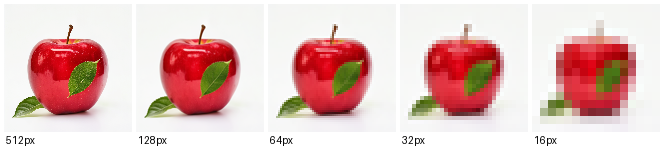
\includegraphics[width=0.95\textwidth]{figures/resolution_comparison.png}
  \caption{The same canonical (``apple,'' generated once by Sana-Sprint and downsampled) at five substrate resolutions: $512$, $128$, $64$, $32$, $16$ pixels per side. The pixel substrate trades off iconic legibility against output-head cost. The toy operates at $64 \times 64$, the smallest resolution that retains the apple's distinguishing structure while keeping the SP's output head from dominating the parameter budget (Table~\ref{tab:resolution}).}
  \label{fig:resolution}
\end{figure}

\begin{table}[ht]
  \centering
  \small
  \begin{tabular}{lrrrr}
    \toprule
    Resolution & Head params & SP total & Head share & Canonicals on disk \\
    \midrule
    $16 \times 16$              & 0.3 M  & 11.4 M & 3\%  & 0.8 MB \\
    $32 \times 32$              & 1.2 M  & 12.2 M & 10\% & 3.1 MB \\
    $\mathbf{64 \times 64}$     & \textbf{4.7 M}  & \textbf{15.8 M} & \textbf{30\%} & \textbf{12.6 MB} \\
    $128 \times 128$            & 18.9 M & 29.9 M & 63\% & 50.3 MB \\
    $256 \times 256$            & 75.5 M & 86.6 M & 87\% & 201 MB \\
    $512 \times 512$            & 302 M  & 313 M  & 96\% & 805 MB \\
    \bottomrule
  \end{tabular}
  \caption{Parameter and storage scaling of the toy across pixel-substrate resolutions, with the transformer body fixed at 6 layers, $d_{\text{model}}=384$. ``Canonicals on disk'' is the full per-word canonical set (1024 images, uint8). The head share is the fraction of the SP's parameters consumed by the pixel-projection head; above $128 \times 128$ the model is mostly head. The toy uses $64 \times 64$ (bold).}
  \label{tab:resolution}
\end{table}

Training has two steps. \textbf{Step 1:} train the SP alone --- a causal transformer with a pixel-output head --- to predict the canonical pixel image of the next token from the running text. Loss is per-pixel MSE. \textbf{Step 2:} freeze the SP; sample next-token contexts and project only its final-position pixel output for each context; train TR-S (a small CNN with BatchNorm) with cross-entropy to map those outputs to the correct next token. TR-S thus tunes to the SP's actual output distribution rather than to the idealized canonical distribution --- inference-time and training-time inputs match exactly. The toy uses a strictly sequential pipeline, simpler than the joint or lockstep variants §3 entertains.

Phase 0 rendered the 1,021 lexical canonicals at approximately 50 seconds per image via Sana-Sprint on the M4's MPS backend and added three fixed special-token placeholders, totalling approximately 14 hours as a one-time preprocessing step. In the reported run, step 1 completed an epoch-equivalent token budget sampled as random windows with replacement (21,877 optimizer steps, batch 16, context 128) in 48 minutes. Step 2 processed 100,000 sampled next-token contexts (12,500 optimizer steps, batch 8) in 5 minutes 19 seconds. With canonicals already cached, the pixel half of the experiment therefore trained in approximately 53 minutes.

\subsection{Text-Description-Substrate Implementation}

The text-description substrate uses the same authored descriptions but encodes them rather than rendering them. In the intended design, this medium keeps ordered roles, relations, mechanisms, and consequences available where literal depiction is strained; the toy tests only fixed encoded targets. A frozen text encoder (\texttt{all-MiniLM-L6-v2} \cite{sbert2019} in the toy; small on disk, runs across the full vocabulary in seconds) maps each description to a fixed-length sequence of per-token hidden states, e.g. $L{\times}d_{\text{enc}}$ with $L=56$ and $d_{\text{enc}}=384$ in the toy. The full sequence is retained rather than mean-pooled into one global sentence vector because pooling would collapse word order and argument binding, the structure the text medium is intended to preserve. Padded positions are filled with a single fixed unit-norm PAD vector from the encoder's padding-token embedding. Every slot in the $L{\times}d_{\text{enc}}$ substrate therefore has a supervised target, either a contextual token state or the shared PAD direction. These per-token encoder-state sequences are the phase-0 canonicals the SP will learn to emit. The architectural shape is identical to the pixel variant: the SP reads running text and emits a per-position substrate state; the TR reads substrate states and emits a token. The only differences are (i) the head: rather than projecting to $3{\times}64{\times}64 = 12{,}288$ pixels, the SP broadcasts its hidden state $h(x) \in \mathbb{R}^{d_{\text{model}}}$ across the $L$ description slots, adds a learned per-slot embedding $e_j$, and applies one \emph{shared} projection $W \in \mathbb{R}^{d_{\text{enc}} \times d_{\text{model}}}$, so slot $j$ emits
\[
  g_j(x) \;=\; \frac{W\,\mathrm{LN}\!\left(h(x) + e_j\right)}{\bigl\lVert W\,\mathrm{LN}\!\left(h(x) + e_j\right)\bigr\rVert}.
\]
The slot embeddings are what make the $L$ outputs distinct; a shared projection alone would emit the same vector at every position. This costs $d_{\text{model}} \cdot d_{\text{enc}} + L \cdot d_{\text{model}} \approx 169$K parameters instead of the $d_{\text{model}} \cdot L \cdot d_{\text{enc}} \approx 8.3$M a full projection to the flattened sequence would need, which is why the description SP is the smaller of the two at 11.3M; (ii) the loss: cosine distance or MSE over the full encoder-state sequence rather than per-pixel MSE; (iii) TR-S's architecture: a small transformer reader over the $L{\times}d_{\text{enc}}$ sequence rather than a CNN over a pixel grid. In the current toy TR-S adds a learned class token and positional embeddings, applies a one-layer bidirectional transformer encoder over the substrate sequence, and maps the class state to vocabulary logits. It receives no story-context tokens and no target-derived attention mask; PAD is represented only by its fixed vector direction inside the substrate. The description SP is somewhat smaller than the pixel variant --- 11.3M parameters against 15.8M --- and avoids the large categorical softmax that an explicit English-token substrate would require.

A second code channel is \emph{length}. Content occupies a mean of 38.6 of the 56 positions, so roughly a third are PAD; because each word has one fixed canonical, the content/PAD boundary exposes description length, and withholding an explicit attention mask from TR-S does not close this channel, since the repeated PAD direction makes the mask inferable. Length is not by itself identifying: the vocabulary spans only 39 distinct lengths, about 5.3 bits against the 10 bits needed to name one of 1024 classes, so it narrows the candidate set rather than determining it. The gap between content-only and PAD-inclusive cosine similarity in the reported run (§8.5) nonetheless shows that PAD prediction is a substantial share of the regression objective.

A third channel that cosine training would otherwise open is closed by construction. Cosine distance is scale-invariant, so a predictor trained under it leaves emitted magnitudes free, and 56 class-dependent norms would be readable by the TR without any deviation in direction. In this implementation the SP applies an explicit unit normalization to every emitted position before the seam, so all magnitudes are one and no norm information crosses it. Implementations that omit that normalization must treat per-position norms as a further leakage channel and probe it directly. Diagnosing this channel requires a length-only classifier, a condition with content states replaced by noise but PAD positions preserved, length-equalized or shift-randomized padding, PAD masked out of both losses, order-shuffled content states, and a mean-pooled baseline. Until those run, the description result should be read as encoded canonical-sequence prediction, not as evidence that sequence order or argument binding is doing work.

Training again proceeds in two steps after phase 0. \textbf{Phase 0:} encode the 1,021 authored descriptions and three fixed special-token sentinel strings through the frozen text encoder and cache the per-token hidden states plus a diagnostic attention mask. This deterministic, non-learning step completes in seconds. Padding is materialized as the same fixed PAD vector in every padded slot, so the substrate is fully specified at all $L$ positions. \textbf{Step 1:} train the SP to predict the encoded-description sequence of the next token's canonical from the running text. Loss is cosine distance over all $L$ positions; the attention mask is used only for diagnostic metrics that separate content-token error from PAD-slot error. \textbf{Step 2:} freeze the SP; sample the same next-token contexts used by the pixel variant and project only its final-position sequence for each context; train TR-S with cross-entropy to map those sequences to the correct next token. TR-S never receives the corpus prefix itself: its only input is the SP's noisy substrate sequence. Evaluation reports frequency baselines and top-$k$ accuracy on SP outputs, since beating random is not an informative bar for a 1024-way Zipfian vocabulary.

Phase 0 completes in seconds to minutes (frozen-encoder forward passes). In the reported run, step 1 completed the same epoch-equivalent token budget sampled as random windows with replacement (87,508 optimizer steps, batch 4, context 128) in 1 hour 49 minutes; step 2 processed the matched 100,000 contexts in 4 minutes 33 seconds. Excluding cached phase-0 construction, the six recorded stages of the two-medium run took a total of 2 hours 47 minutes on the M4 MPS backend.

\subsection{Comparison and Discussion}

The comparison concerns structured continuous description encodings and structured continuous pixels. The two media share the training corpus and evaluation contexts; within each readout scope, their sampled readout-training windows are also shared. Their SP and TR modules are medium-specific. Two SP differences are quantitative and pull in opposite directions. The pixel SP is the larger model (15.8M parameters, 4.7M of them in the pixel head) against the description SP's 11.3M; but it consumed the identical epoch-equivalent token budget in 21,877 optimizer steps at batch 16, against the description SP's 87,508 steps at batch 4 --- four times fewer gradient updates. The reported ordering therefore rests on a capacity advantage for pixels and an update-count advantage for descriptions, neither of which is controlled. A result for one medium measures the complete medium-specific pipeline, not a perfectly isolated causal effect of geometry. Attributing a difference specifically to geometric structure requires stronger controls.

A further limitation applies to both media: the pilot's output heads are single dense projections from one transformer state, trained with coordinatewise losses. For any fixed permutation $P$ of output coordinates, $\lVert PWh - Pv\rVert^2 = \lVert Wh - v\rVert^2$, so nothing in the SP's architecture or objective distinguishes the true pixel arrangement from an arbitrary fixed shuffling of it; the same holds across the description sequence's positions. The medium's geometry is thus a property of the \emph{targets} and of TR-S's inductive bias (the CNN sees locality; the sequence reader sees order), not something the SP's computation must respect. It is useful to separate a \emph{target-shaped interface} --- the output tensor can be displayed as an image or read as a sequence --- from a \emph{medium-respecting predictor}, whose computation is constrained by locality, translation, or ordering (a convolutional, latent-grid, or diffusion decoder; a shared sequence decoder). The pilot establishes the former; testing rendering pressure (§1) requires the latter.

\subsection{Pilot Experiment and Results}

\paragraph{Protocol.} The reported run uses seed 42, the first 250,000 TinyStories \cite{tinystories2023} records, a 1024-token vocabulary, and context length 128. Tokenization produces 44,812,714 tokens, of which 9.0\% are \texttt{<unk>}. Each SP is trained for an epoch-equivalent token budget using random windows sampled with replacement: 21,877 optimizer steps at batch 16 for the pixel SP, 87,508 steps at batch 4 for the description SP. Each TR-S is then trained against its frozen SP on the same 100,000 sampled contexts with batch size 8 and evaluated on the same 1024 deterministic, evenly spaced contexts from a disjoint 8192-token holdout stream. Even spacing places these contexts roughly eight tokens apart while each carries a 128-token window, so neighboring examples overlap heavily and are not independent; the effective sample size is far below 1024. TR-S receives only the SP's final emitted substrate state. The training pipeline requires a completed SP checkpoint before the readout stage begins, so no TR is fitted to a partially trained predictor. The run is recorded as \texttt{data5x\_seed42}.

The derived TR-C run \texttt{tr\_c\_data5x\_seed42\_t128} reuses the frozen pixel and description SP checkpoints from \texttt{data5x\_seed42}. The TR-S checkpoints are re-evaluated only as comparators; they neither initialize nor participate in TR-C. For each of 100,000 deterministically sampled length-128 windows, shared across media, the frozen SP emits its causal state at every position. A freshly initialized medium-specific adapter, shared across positions within its medium, independently maps each state to 256 dimensions. A two-layer, eight-head causal Transformer reads the complete sequence including the current state and emits vocabulary logits at every position. Training uses batch size 8 and same-index cross-entropy against all 128 aligned next-token targets, for 12.8 million supervised positions per medium and 12,500 optimizer updates. Source-token IDs and SP hidden states are inputs only to the frozen SP and never to TR-C. Evaluation uses the identical 1024 held-out contexts and reports final-position NLL and top-$k$ metrics, so each TR-C result is evaluated on the same outcomes as its medium's TR-S result. The immutable manifest binds the source SP, TR-S, and direct-token checkpoint hashes; dataset and encoder revisions; token-stream, vocabulary, and canonical hashes; window-sampling and initialization seeds; model and optimizer settings; software versions; and output checkpoint and metrics hashes. Its compact result and provenance record accompany the code.

For provenance, the local Hugging Face cache used by these runs contains a single TinyStories snapshot, commit \texttt{f54c09fd2331}; rebuilding both corpus slices from that immutable revision reproduces their exact token counts. The accompanying reproduction record binds each slice further by a SHA-256 hash of its complete token-ID stream and records hashes for the vocabulary, canonical tensors, metrics, and checkpoints. The runner pins the dataset and encoder revisions and fails closed on any input-identity mismatch. The reproduction record supplements the run manifests with the dataset revision and hashes. Saved-checkpoint evaluation is deterministic and reproduces the recorded metrics.

Table~\ref{tab:pilot-results} also reports an earlier run at one fifth of this data budget (\texttt{paper\_seed42\_e1\_n2-100k}, 8,826,412 tokens), which uses the same protocol, seed, and canonicals with only the corpus slice changed. Its holdout stream is the tail of a shorter slice and therefore a different text with different token frequencies, so the two runs are compared by margin over their own baselines rather than by raw accuracy.

\begin{table}[ht]
  \centering
  \small
  \begin{tabular}{llrrrr}
    \toprule
    System & SP train tokens & Eval.\ NLL & Top-1 & Top-5 & Top-10 \\
    \midrule
    Context-free frequency baseline & 44.8M & --    & 8.1\%           & 27.2\%           & 39.5\% \\
    Direct-token LM (backbone-matched) & 44.8M & \textbf{2.208} & \textbf{44.7\%} & \textbf{74.6\%} & \textbf{85.3\%} \\
    Description SP + TR-C      & 44.8M & 2.616 & 41.9\%          & 68.6\%           & 78.0\% \\
    Pixel SP + TR-C            & 44.8M & 2.954 & 37.8\%          & 61.6\%           & 72.2\% \\
    Description SP + TR-S      & 44.8M & 3.541 & 35.0\%          & 54.2\%           & 62.8\% \\
    Pixel SP + TR-S            & 44.8M & 4.283 & 27.8\%          & 44.3\%           & 52.9\% \\
    \midrule
    Context-free frequency baseline & 8.8M  & --    & 11.0\%          & 27.4\%           & 39.7\% \\
    Description SP + TR-S      & 8.8M  & 3.998 & 29.7\%          & 47.9\%           & 56.1\% \\
    Pixel SP + TR-S            & 8.8M  & 4.466 & 22.0\%          & 40.1\%           & 50.3\% \\
    \bottomrule
  \end{tabular}
  \caption{Next-token results on 1024 held-out contexts. Within each budget all rows use the same holdout. The 44.8M-token block is the five-configuration comparison: TR-C reuses the frozen SPs but is freshly trained with a different architecture and 12.8M aligned labels per medium, versus 100,000 final-position labels for TR-S, so TR-C--TR-S differences do not isolate history. Across budgets the holdout differs, which is why the frequency baseline moves. All percentage-point differences discussed below are computed from the unrounded accuracies. The context-free baseline always predicts the $k$ most common holdout targets; it is an oracle test-marginal reference, not a deployable model or a mathematical floor. Each trained condition is one seed; no confidence intervals are claimed.}
  \label{tab:pilot-results}
\end{table}

\paragraph{Feasibility result.} All four substrate configurations substantially exceed the context-free frequency baseline at 44.8M tokens. TR-S reaches 35.0\% top-1 for descriptions and 27.8\% for pixels, establishing that the current SP output alone carries context-dependent next-token information. TR-C reaches 41.9\% and 37.8\%, improvements of 6.9 and 10.0 points over the corresponding TR-S conditions on the identical holdout. Because neither readout has source-token access, the emitted state or trace is sufficient for a separate reader to recover useful predictive signal. The gain does not isolate temporal memory, and none of these results shows that the SP exploited the intended meaning of the targets; fixed canonicals may function as learnable codewords.

\paragraph{Direct-token baseline.} A backbone-matched direct-token language model --- matching the pixel SP's causal transformer body, corpus slice, seed, batch size, optimizer, learning rate, and 21,877 optimizer steps, but with an ordinary token-softmax head and no seam or TR --- reaches 44.7\% top-1 and 2.208 next-token NLL (perplexity 9.1) on the same 1024 holdout contexts. It shares the transformer body, corpus slice, and seed with the description SP, whose batch size and update count differ as reported above. The baseline is recorded as \texttt{baseline5x\_seed42}. Against TR-S it leads descriptions by 9.8 top-1 points and pixels by 16.9; against TR-C the gaps narrow to 2.8 and 6.9 points. Perplexity is 9.1 for the direct model, 13.7 and 19.2 for description and pixel TR-C, and 34.5 and 72.5 for TR-S. The direct system has 11.48M parameters; TR-C adds 2.66M parameters to the description SP and 1.93M to the pixel SP and receives 12.8M position labels per medium. Total FLOPs were not measured. These numbers rank the reported configurations but do not estimate a causal cost for the seam. The baseline does not test context-dependent scene targets, so its lead weighs against H1's parity subprediction only for the present implementation.

The run using a five-times larger corpus slice records higher values on every reported metric, with code, seed, and canonicals held fixed. Top-1 margins over each run's own frequency baseline are 26.9 rather than 18.7 points for descriptions and 19.7 rather than 10.9 for pixels; TR-S cross-entropy is 3.541 rather than 3.998 and 4.283 rather than 4.466. The pixel SP's evaluation MSE is 17\% lower (0.0483 rather than 0.0582), and the description SP's content-position cosine similarity is 0.417 rather than 0.379. The larger run sees roughly 2.83 tokens per SP parameter for pixels and 3.98 for descriptions (2.45 and 3.26 if TR-S is counted), far below the roughly twenty-tokens-per-parameter regime reported for much larger conventional transformers \cite{chinchilla2022}; whether that heuristic transfers here is unknown. Both continuations remain degenerate, and further training could improve, plateau, or degrade generalization.

This pattern is consistent with the smaller run being budget-limited, but the two-point comparison is not a causal estimate or a clean learning curve. Each run's holdout is the tail of its own corpus slice, so the evaluations differ in text and intrinsic difficulty; comparing margins over each run's own baseline mitigates but does not control for that. A proper budget comparison evaluates both checkpoints on identical frozen contexts, which for these runs means using the larger run's holdout: the smaller run's holdout lies inside the larger run's training stream, so the reverse direction would score a model on text it was trained on.

Across media, the text-description substrate is stronger at every reported cutoff and with both readout scopes. Under TR-S it exceeds pixels by 7.1 top-1 points; under TR-C the gap is 4.1 points. The SP regression diagnostics are not directly comparable across media: the description SP reaches 0.417 content-position cosine similarity (0.482 including PAD positions), while the pixel SP reaches MSE 0.0483. The evidence therefore favors the description pipeline as an information channel in this particular toy. Without each medium's shuffled and random controls, the difference cannot be attributed to ordered semantic structure, spatial geometry, or meaningfulness generally. The pilot trains pixels in a fixed-canonical MSE regime expected to be unfavorable to crisp conditional images. The pixel medium's hypothesized advantage --- rendering pressure that forces scene assembly (§1) --- arises, if at all, under generative, context-conditioned objectives at scale, a regime this pilot does not reach. The ordering therefore applies only to these two small pipelines under fixed-canonical regression; the space of candidate media remains open (video, audio, and hybrid substrates; §9).

\paragraph{Qualitative output.} From the prompt ``the dog ran into the yard,'' the text variant continues ``it was and it was and it was and it was it was and,'' while the detokenized pixel continuation gives ``and was the and and.'' Both strips also contain \texttt{<unk>} predictions that the detokenizer suppresses. These labels are the expected degenerate predictions rather than anything substrate-specific: \texttt{<unk>} is the corpus's single most frequent target (9.0\% of tokens) and ``and'' is among the top function words, and an undertrained model facing next-token uncertainty falls into exactly this high-frequency loop in either medium.

The pixel strip changes qualitatively in the larger-corpus run, which narrows a confound the smaller run left open. At 8.8M tokens every emitted state was the same gray-brown average, consistent both with the regression-to-the-mean effect §3 predicts for fixed-target training and with simple undertraining. At 44.8M tokens the early positions are visibly differentiated and partly recognizable: Figure~\ref{fig:pilot-pixel-strip} contains a dog-like state, a face-like state, and a distinct red vertical element, before later positions decay into the earlier uniform blur. This pattern is consistent with undertraining contributing to the smaller-run collapse, but the runs use different holdout text and therefore do not identify the cause. The residual decay is also consistent with degenerate generation contributing: once the emitted text enters the \texttt{and}/\texttt{<unk>} loop, the predictor conditions on its own repetitive prefix, so its predicted target distribution can also repeat.

Two cautions attach to this improvement. First, legibility is not yet fidelity: the decoded tokens do not match what a human reads in the states, and a state that strongly resembles the vocabulary's authored dog canonical is decoded as \texttt{<unk>}. Because this is a free-running continuation, there is no ground-truth next token at that position; visual resemblance also does not establish that the SP emitted the correct canonical or that TR-S alone is at fault. This sample establishes only that human-recognizable dog-like structure and machine decodability can diverge. The mismatch is consistent with TR-S reading artifact dimensions rather than gross content, but equally with an off-canonical dog, with insufficient readout invariance to a narrow output distribution, or with an ordinary class-boundary error. Separating these requires the aggregate intervention of the channel-versus-manifold readout comparison (§9), not inspection of individual frames. Second, the qualitative sample remains a failure analysis, not evidence of coherent generation.

\begin{figure}[ht]
  \centering
  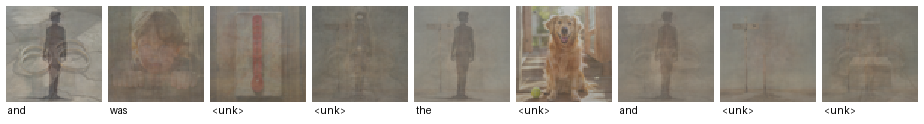
\includegraphics[width=\textwidth]{figures/pilot_pixel_strip_5x.png}
  \caption{The first nine pixel-substrate states emitted after the prompt ``the dog ran into the yard'' in the 44.8M-token run, labelled with TR-S's decoded tokens. Unlike the smaller run, in which every state was the same gray-brown average, several early states are differentiated and partly recognizable --- a dog-like state in the sixth position, a face-like state in the second, a red vertical element in the third --- before later positions decay toward uniform blur as the generated text enters its \texttt{and}/\texttt{<unk>} loop. The decoded tokens do not correspond to what a human reads in the states: the dog-like state is decoded as \texttt{<unk>}. This is an unaltered crop of the run's substrate-state strip.}
  \label{fig:pilot-pixel-strip}
\end{figure}

The text-description substrate is less directly inspectable than an explicit English-token sequence but more diagnostically accessible than an unstructured latent: nearest-neighbour lookup can be applied per encoder position or over whole canonical sequences to approximate what region of description space the SP has entered. This is a research aid, not the substrate's purpose. The pixel variant is directly displayable, but displayability is not the same as interpretability, as Figure~\ref{fig:pilot-pixel-strip} shows.

\subsection{Limitations}

The toy deliberately uses one fixed canonical per word and trains both readouts on actual SP outputs. This simplifies fidelity analysis while enabling fixed-code and artifact shortcuts; raw pixels and frozen description states likewise support medium-specific probes but do not capture higher-dimensional reconstruction latents.

\paragraph{Scope of the evidence.} The pilot supports only narrow causal and comparative conclusions. It contains no accumulating scene, uses one seed per condition and two corpus budgets with different holdout text, maps 9.0\% of tokens to \texttt{<unk>}, and evaluates on heavily overlapping contexts (§8.5). It has no uncertainty estimates, capacity- and compute-matched direct-token baseline, shuffled or random-target control, earlier-state intervention, or targeted spatial/coherence benchmark; its media and readouts also differ in dimensions, losses, capacity, updates, and supervision density. Future runs should split by story, sample non-overlapping contexts, report accuracy excluding \texttt{<unk>} and by token-frequency bin, and prefer a tokenizer without a large out-of-vocabulary class. These are single-seed, plausibly budget-sensitive configuration estimates, not lower bounds.

\section{Future Work}

\paragraph{Immediate validation.} Validation should proceed in two stages before video or frontier scale. First, estimate $\Delta_{\mathrm{meaning}}$ using fixed permutations under the present design (§8.1). Second, multi-prototype or context-selected canonicals (§2) should replace the atomic one-image-per-word mapping, so that a word maps to a cloud of instances and structure within and across those clouds becomes something the model can exploit. Meaning has far more opportunity to become load-bearing there, and the same permutation control becomes a correspondingly sharper test.

The minimum design begins with a matched direct-token LM. Within each substrate medium, aligned, shuffled, and random targets must use identical training data, sampled contexts, holdout, architecture, and optimizer-update count, so that no condition receives more gradient steps than another (§8.4). Readout decodability must also be matched, so that an easy codebook does not masquerade as a semantic effect.

Paired aligned and shuffled runs should share initialization and data order, and they should be crossed with multiple independently sampled fixed permutations that keep special-token targets fixed. At least three training seeds, per-example predictions, and uncertainty intervals are required. Evaluation should pair ordinary language loss with a controlled compositional or configurational benchmark. For descriptions, it should also include the name-only, masked-name, and name-free leakage conditions of §8.1 together with the padding and length ablations of §8.3.

Each condition should be evaluated under two readout-training regimes: a \emph{channel readout} trained on the SP's outputs as in the pilot, and a \emph{manifold readout} trained on canonical content with meaningful within-concept variation and frozen before evaluation. The latter needs several instances per word where available, not merely perceptual jitter, which would leave it a memorized lookup rather than a semantic reader. The channel readout should score higher by construction, since it sees the SP's actual output distribution and may exploit artifacts. The informative quantity is the gap rather than either level: a small gap means the SP's emissions sit near the authored canonicals, while a large one means the decodable information lives in artifacts rather than in the intended content.

Together these comparisons estimate three distinct quantities: alignment, from aligned versus shuffled and random targets under matched adaptive readouts; fidelity, from the frozen manifold readout; and utility, from the matched direct-token LM. Because a permutation preserves target-set geometry and changes only the word-to-target assignment, any one-way decoder-adaptation advantage remains available in both aligned and shuffled conditions, making $\Delta_{\mathrm{meaning}}$ under matched adaptive readouts the primary alignment estimator. The frozen reader cannot by itself establish that meaning is load-bearing, and an aligned advantage visible only under the adaptive reader would indicate decoder adaptation or artifact exploitation rather than fidelity. A conditional or generative pixel objective with a medium-respecting decoder (§8.4) should then test whether crisp, context-specific scenes create stronger rendering pressure than the present fixed-canonical regression; for pixels, decoding robustness under compression, blur, quantization, and added noise separates recognizable content from machine-readable residue.

Positive stage-1 controls would justify testing whether short-video representations built from the spatiotemporal latents of a frozen video autoencoder outperform matched still-image controls before attempting persistent state. Evidence at that stage would in turn justify Stage 3's revisable physical-and-schematic scene and interventions against recurrent private code. That implementation likely requires collaboration with the world-model and video-generation communities; frontier-scale resources should follow controlled stage-1 and stage-2 results, not feasibility alone.

\paragraph{Tokenization at scale.} The pilot uses a 1024-token vocabulary whose 1,021 lexical entries are whole words, but production models operate on subword fragments, punctuation, whitespace variants, and bytes, many of which denote nothing on their own; there is no canonical image of a suffix or a formatting token. This challenges one-substrate-object-per-token directly, and it is a design problem rather than an implementation detail. Candidate resolutions: word-level substrate generation with a subword or character spelling decoder beneath it; emitting substrate states only at semantic-unit boundaries; predicting multi-token lexical units or concepts, as in next-concept prediction \cite{nextconcept2026}; or letting the TR map one substrate state to a variable-length token sequence. Which of these preserves the no-bypass property without reintroducing a token-statistics pathway is open.

\paragraph{Encoder family and spatial structure.} The choice of encoder family is the program's most consequential pre-training decision: \emph{the substrate must have an explicit spatial axis}. A single global vector --- the output of contrastive encoders like CLIP, SigLIP, EVA-CLIP --- has no $(x, y)$ coordinates internal to it. Contrastive training was caption-discriminative, and captions usually say what is in an image rather than precisely where, so such encoders plausibly attenuate fine spatial detail their objective did not require. Global-vector substrates therefore lack an explicit, displayable spatial axis --- some spatial relations may remain probe-decodable inside them, but not as inspectable $(x,y)$ structure. \emph{Reconstruction} latents --- the spatially-structured grids of feature vectors inside FLUX, Stable Diffusion 3, and masked autoencoders --- preserve a spatial axis because they have to be decodable back to pixels. Raw pixels preserve the spatial axis natively, at the cost of higher dimensionality. An explicit spatial axis in the target is nonetheless only a precondition: §8.4 shows that it does not by itself make the predictor's computation respect that geometry. Accordingly, this program selects substrates with explicit spatial indexing; spatial information recoverable from global contrastive vectors does not satisfy that design criterion.

At each stage, the borrowed visual and video encoders are optimized for visual or video generation, not for downstream language modeling. A natural extension is to train encoders specifically for the architecture, with compression profiles tuned for language modeling while remaining decodable for the fidelity probes under H3.

The trajectory also generalizes beyond vision. An audio substrate (text-to-audio encoder at stage 1, audio sequences at stage 2, persistent audio scene at stage 3) would test whether prediction can be mediated by sound-structured working states. An embodied substrate (text-to-action) would test the same hypothesis with motor-plan structure. The vision-and-video case is the one the necessary encoders most clearly support today; other modalities follow as their encoders mature.

\section*{Code and Reproducibility}

Code, paper source, vocabulary metadata, immutable run manifests, compact metrics, and per-example TR-C predictions accompany the paper at \url{https://github.com/emergent-wisdom/substrate-language-modeling}. Canonical target tensors and images, together with the exact eleven checkpoints across the four reported run IDs, are hosted in the companion artifact repository at \url{https://huggingface.co/emergent-wisdom/substrate-language-modeling}. The tracked release records and the artifact repository's \texttt{SHA256SUMS} manifest identify released files by path, byte size, and SHA-256 digest.

The run manifests bind every reported configuration to its authenticated inputs, training settings, and artifact hashes. Exact saved-checkpoint evaluation reproduces the reported TR-S measurements at full precision; the TR-C prediction files reproduce top-$k$ counts exactly and NLL within $10^{-7}$, the tolerance needed after serializing per-example float32 log probabilities. Fresh training from frozen inputs is pinned and seeded, although Apple MPS does not guarantee bitwise-identical training across hardware or software versions. The two repositories therefore support both external use of the authors' exact checkpoint bytes and independent training replication from authenticated inputs.

\section{Conclusion}

The long-term STLM hypothesis is a model that builds a world as it writes: a persistent configurational scene that accumulates interacting physical and schematic structure and is the sole lexical interface. This paper implements only its stage-1 prerequisite: a compulsory no-bypass interface with independent per-position image and description targets.

In the reported TinyStories comparison, both media transmit useful next-token signal through both readout scopes, but the direct-token model remains best. The causal readouts narrow the gap without isolating memory because architecture, capacity, and supervision density change together. The pixel strip also separates human-legible content from machine decoding. These results establish the compulsory seam, not load-bearing meaning or scene emergence.

The decisive next test is whether intended word-to-image and word-to-description mappings beat fixed permutations under matched capacity, supervision, and readout decodability, especially on compositional and structure-sensitive tasks. Positive stage-1 alignment, fidelity, and composition evidence is required before progressing through event-shaped substrates to the persistent scene. Once that scene exists, controlled state edits must show that its intended organization causes corresponding behavioral changes. An accumulating, manipulable world built from reusable meaningful structure rather than private codes --- not merely an expensive code channel --- is the criterion for scene emergence.

\begin{thebibliography}{99}

\bibitem{talespin1977} J. R. Meehan. TALE-SPIN, An Interactive Program that Writes Stories. \emph{Proceedings of the 5th International Joint Conference on Artificial Intelligence (IJCAI)}, pp. 91--98, 1977.

\bibitem{dynamicentities2023} J. Guan, Z. Yang, R. Zhang, Z. Hu, and M. Huang. Generating Coherent Narratives by Learning Dynamic and Discrete Entity States with a Contrastive Framework. \emph{Proceedings of the AAAI Conference on Artificial Intelligence}, 37(11):12836--12844, 2023.

\bibitem{imagineverbalize2022} P. Wang, J. Zamora, J. Liu, F. Ilievski, M. Chen, and X. Ren. Contextualized Scene Imagination for Generative Commonsense Reasoning. \emph{International Conference on Learning Representations (ICLR)}, 2022.

\bibitem{visualscaffolding2026} B. Mohapatra, G. Duca, L. Romary, and J. Cassell. Using Machine Mental Imagery for Representing Common Ground in Situated Dialogue. \emph{arXiv:2604.21144}, 2026.

\bibitem{orca2026} Y. Wang et al. Orca: The World is in Your Mind. \emph{arXiv:2606.30534}, 2026.

\bibitem{cbm2020} P. W. Koh et al. Concept Bottleneck Models. \emph{ICML}, 2020.

\bibitem{cbllm2024} C.-E. Sun, T. Oikarinen, and T.-W. Weng. Crafting Large Language Models for Enhanced Interpretability. \emph{ICML Mechanistic Interpretability Workshop / arXiv:2407.04307}, 2024.

\bibitem{cbplm2024} A. A. Ismail et al. Concept Bottleneck Language Models for Protein Design. \emph{arXiv:2411.06090}, 2024.

\bibitem{cbmleakage2022} M. Havasi, S. Parbhoo, and F. Doshi-Velez. Addressing Leakage in Concept Bottleneck Models. \emph{NeurIPS}, 2022.

\bibitem{lcm2024} LCM Team et al. Large Concept Models: Language Modeling in a Sentence Representation Space. \emph{arXiv:2412.08821}, 2024.

\bibitem{calm2025} C. Shao et al. Continuous Autoregressive Language Models. \emph{arXiv:2510.27688}, 2025.

\bibitem{projectedar2026} O. Naparstek. Projected Autoregression: Autoregressive Language Generation in Continuous State Space. \emph{arXiv:2601.04854}, 2026.

\bibitem{vmf2019} S. Kumar and Y. Tsvetkov. Von Mises--Fisher Loss for Training Sequence to Sequence Models with Continuous Outputs. \emph{ICLR}, 2019.

\bibitem{ecoc2019} J. O'Neill and D. Bollegala. Error-Correcting Neural Sequence Prediction. \emph{arXiv:1901.07002}, 2019.

\bibitem{nextconcept2026} Y. Liu et al. Next Concept Prediction in Discrete Latent Space Leads to Stronger Language Models. \emph{arXiv:2602.08984}, 2026.

\bibitem{vokenization2020} H. Tan and M. Bansal. Vokenization: Improving Language Understanding with Contextualized, Visual-Grounded Supervision. \emph{EMNLP}, 2020.

\bibitem{valm2022} W. Wang et al. Visually-Augmented Language Modeling. \emph{ICLR}, 2023.

\bibitem{inlg2023} W. Zhu et al. Visualize Before You Write: Imagination-Guided Open-Ended Text Generation. \emph{Findings of EACL}, 2023.

\bibitem{live2023} T. Tang et al. Learning to Imagine: Visually-Augmented Natural Language Generation. \emph{ACL}, 2023.

\bibitem{blindvalm2025} P. Ontalvilla, A. Ormazabal, and G. Azkune. Improving the Efficiency of Visually Augmented Language Models. \emph{COLING}, 2025.

\bibitem{silentlvr2026} D. Zhu et al. Leveraging Latent Visual Reasoning in Silence. \emph{arXiv:2605.18641}, 2026.

\bibitem{lecun2022path} Y. LeCun. A Path Towards Autonomous Machine Intelligence. \emph{OpenReview / position paper}, 2022.

\bibitem{ijepa2023} M. Assran et al. Self-Supervised Learning from Images with a Joint-Embedding Predictive Architecture. \emph{arXiv:2301.08243}, 2023.

\bibitem{vjepa2024} A. Bardes et al. Revisiting Feature Prediction for Learning Visual Representations from Video. \emph{arXiv:2404.08471}, 2024.

\bibitem{vjepa2_2025} M. Assran et al. V-JEPA 2: Self-Supervised Video Models Enable Understanding, Prediction and Planning. \emph{arXiv:2506.09985}, 2025.

\bibitem{llmjepa2025} H. Huang, Y. LeCun, and R. Balestriero. LLM-JEPA: Large Language Models Meet Joint Embedding Predictive Architectures. \emph{arXiv:2509.14252}, 2025.

\bibitem{vljepa2025} D. Chen et al. VL-JEPA: Joint Embedding Predictive Architecture for Vision-Language. \emph{arXiv:2512.10942}, 2025.

\bibitem{jepat2025} S. Wan et al. JEPA-T: Joint-Embedding Predictive Architecture with Text Fusion for Image Generation. \emph{arXiv:2510.00974}, 2025.

\bibitem{imagen2022} C. Saharia et al. Photorealistic Text-to-Image Diffusion Models with Deep Language Understanding (Imagen). \emph{NeurIPS}, 2022.

\bibitem{stablediffusion} R. Rombach et al. High-Resolution Image Synthesis with Latent Diffusion Models. \emph{CVPR}, 2022.

\bibitem{pixel2022} P. Rust et al. Language Modelling with Pixels. \emph{ICLR}, 2023.

\bibitem{seeker2024} Y. Lu et al. From Text to Pixel: Advancing Long-Context Understanding in MLLMs (SEEKER). \emph{arXiv:2405.14213}, 2024.

\bibitem{glyph2025} J. Cheng et al. Glyph: Scaling Context Windows via Visual-Text Compression. \emph{arXiv:2510.17800}, 2025.

\bibitem{deepseekocr2026} H. Wei, Y. Sun, and Y. Li. DeepSeek-OCR: Contexts Optical Compression. \emph{arXiv:2510.18234}, 2025.

\bibitem{lvr2025} B. Li et al. Latent Visual Reasoning. \emph{arXiv:2509.24251}, 2025.

\bibitem{mirage2025} Z. Yang et al. Machine Mental Imagery: Empower Multimodal Reasoning with Latent Visual Tokens. \emph{arXiv:2506.17218}, 2025.

\bibitem{flux2024} Black Forest Labs. FLUX.1. Open-weights text-to-image model release, 2024.

\bibitem{fluid2024} L. Fan et al. Fluid: Scaling Autoregressive Text-to-image Generative Models with Continuous Tokens. \emph{arXiv:2410.13863}, 2024.

\bibitem{llamagen2024} P. Sun et al. LlamaGen: Autoregressive Model Beats Diffusion: Llama for Scalable Image Generation. \emph{arXiv:2406.06525}, 2024.

\bibitem{nextstep2025} StepFun NextStep Team. NextStep-1: Toward Autoregressive Image Generation with Continuous Tokens at Scale. \emph{arXiv:2508.10711}, 2025.

\bibitem{latentsketchpad2025} H. Wang et al. Latent Sketchpad: Sketching Visual Thoughts to Elicit Multimodal Reasoning in MLLMs. \emph{arXiv:2510.24514}, 2025.

\bibitem{monet2025} Q. Wang, Y. Shi, Y. Wang, Y. Zhang, P. Wan, K. Gai, X. Ying, and Y. Wang. Monet: Reasoning in Latent Visual Space Beyond Images and Language. \emph{arXiv:2511.21395}, 2025.

\bibitem{svd2023} A. Blattmann et al. Stable Video Diffusion: Scaling Latent Video Diffusion Models to Large Datasets. \emph{arXiv:2311.15127}, 2023.

\bibitem{sora2024} OpenAI. Video Generation Models as World Simulators (Sora technical report), 2024.

\bibitem{tinystories2023} R. Eldan and Y. Li. TinyStories: How Small Can Language Models Be and Still Speak Coherent English? \emph{arXiv:2305.07759}, 2023.

\bibitem{sanasprint2025} J. Chen et al. SANA-Sprint: One-Step Diffusion with Continuous-Time Consistency Distillation. \emph{ICCV / arXiv:2503.09641}, 2025. Checkpoint \texttt{Efficient-Large-Model/Sana\_Sprint\_1.6B\_1024px}.

\bibitem{sbert2019} N. Reimers and I. Gurevych. Sentence-BERT: Sentence Embeddings using Siamese BERT-Networks. \emph{EMNLP}, 2019. Checkpoint \texttt{sentence-transformers/all-MiniLM-L6-v2}.

\bibitem{chinchilla2022} J. Hoffmann et al. Training Compute-Optimal Large Language Models. \emph{arXiv:2203.15556}, 2022.

\bibitem{lakoff_johnson} G. Lakoff and M. Johnson. \emph{Metaphors We Live By}. University of Chicago Press, 1980.

\bibitem{barsalou} L. W. Barsalou. Perceptual symbol systems. \emph{Behavioral and Brain Sciences}, 1999.

\bibitem{paivio} A. Paivio. \emph{Mental Representations: A Dual Coding Approach}. Oxford University Press, 1986.

\end{thebibliography}

\end{document}
